\newpage
\section*{8\quad Learning: how the arrows get nudged}
\addcontentsline{toc}{section}{8 Learning}
\startchapter{8}
\providecommand{\fitR}[1]{\leavevmode\setbox0\hbox{#1}\ifdim\wd0>\linewidth\resizebox{\linewidth}{!}{\box0}\else\box0\fi}

\begin{chaptermap}
Chapter 3 ended with a promise: training turns and stretches the query, key and value arrows until the
model attends to the right words. This chapter keeps that promise. We first need a number that says how
wrong a guess is (\S8.1), then a way to get many such numbers from one sentence (\S8.2). With that number we
can draw a landscape and walk downhill on it (\S8.3), watch the arrows of our toy turn as it learns (\S8.4),
see why real training uses small random batches (\S8.5), and finally train a real, tiny transformer on a corpus
of transcribed technical talks and read what it writes (\S8.6). There is no calculus in this chapter; Appendix A has it
for readers who want it.
\end{chaptermap}

\machine{8}{You are here: the \emph{loss} box at the bottom right. Nothing new is added to the model itself.
This chapter adds the one number that compares the model's guess with the right next word, and the walk downhill
that changes every weight in the solid blocks above it. The dashed blocks come later.}

\begin{beforeyoustart}
\begin{enumerate}[label=(\arabic*),leftmargin=1.6em]
\item What is $0.5\times0.5\times0.5\times0.5$? \emph{Refresher: multiply step by step: 0.25, 0.125,
0.0625. Multiplying numbers below 1 makes them smaller every time.}
\item The natural logarithm $\ln x$ answers ``$e$ to what power gives $x$?''. What is $\ln 1$? Is $\ln 0.5$
positive or negative? \emph{Refresher: $e^0=1$, so $\ln 1=0$. Since $e^{\text{negative}}$ is below 1,
the log of any number between 0 and 1 is negative: $\ln 0.5\approx-0.693$.}
\item Logs turn multiplying into adding: $\ln(a\times b)=\ln a+\ln b$. Check it with $a=b=e$.
\emph{Refresher: $\ln(e\cdot e)=\ln e^2=2=1+1$.}
\item You stand on a slope in thick fog. You step one foot left and feel the ground go down. Which way do
you walk? \emph{Refresher: left. You do not need to see the valley; you need the slope under your feet.}
\end{enumerate}
\end{beforeyoustart}

%---------------------------------------------------------------------
\subsection*{8.1\quad How wrong is a guess? Surprise}

\Predict Our toy reads \tok{waste of time} and must guess the next word. The right answer is
\tok{Sorry}. Suppose the model gives \tok{Sorry} a probability of 15\%. Before reading on, write down how
you would score that guess. Is it ``wrong'' because another word got more? Is it ``85\% wrong''?

Let us first see what our toy actually says. Take the attention output for \tok{time} from Chapter 3,
$\bm{o}_{\text{time}}=\nEightOTime$. To turn it into a score for every word in the 12-word toy vocabulary,
we take its dot product with every word's own embedding arrow (the same table $E$ that gave the words their
arrows; reusing it is called \emph{tying}, and Chapter 7 explains why it is reasonable). Then softmax turns the 12 scores into shares, exactly as in \S3.7. Figure~\ref{fig:ch8scores} shows the whole calculation as matrices.

\begin{figure}[!tbp]
\centering
\fitR{% AUTO-GENERATED by code/figlib.py helpers -- do not edit
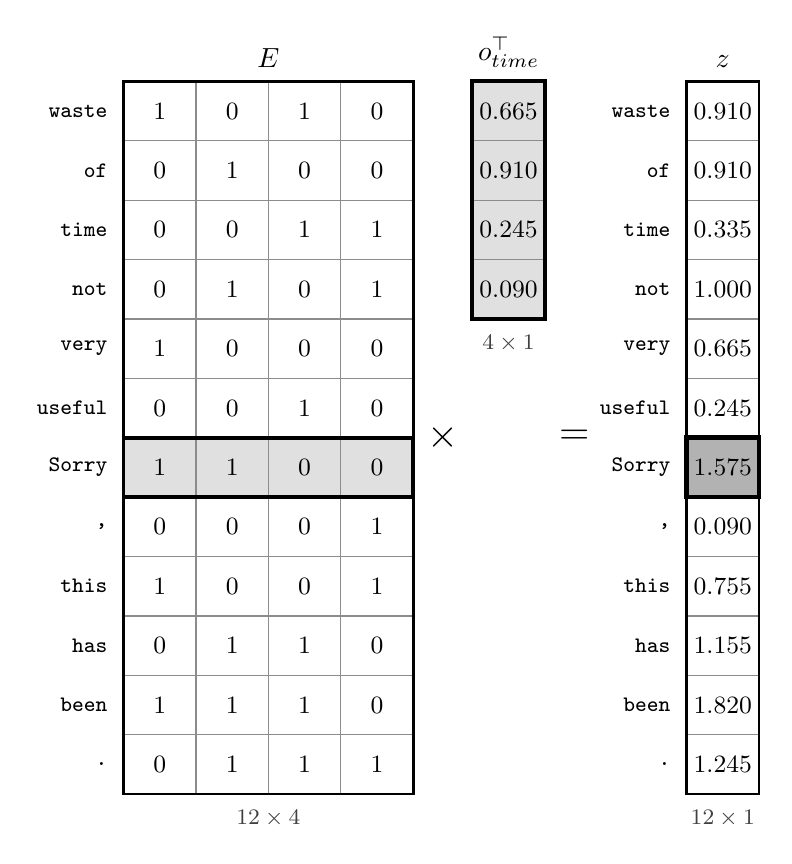
\begin{tikzpicture}
\draw[black!45, fill=white] (0.000,0.000) rectangle (0.920,-0.754);
\node[font=\small, text=black] at (0.460,-0.377) {$1$};
\draw[black!45, fill=white] (0.920,0.000) rectangle (1.840,-0.754);
\node[font=\small, text=black] at (1.380,-0.377) {$0$};
\draw[black!45, fill=white] (1.840,0.000) rectangle (2.760,-0.754);
\node[font=\small, text=black] at (2.300,-0.377) {$1$};
\draw[black!45, fill=white] (2.760,0.000) rectangle (3.680,-0.754);
\node[font=\small, text=black] at (3.220,-0.377) {$0$};
\draw[black!45, fill=white] (0.000,-0.754) rectangle (0.920,-1.509);
\node[font=\small, text=black] at (0.460,-1.132) {$0$};
\draw[black!45, fill=white] (0.920,-0.754) rectangle (1.840,-1.509);
\node[font=\small, text=black] at (1.380,-1.132) {$1$};
\draw[black!45, fill=white] (1.840,-0.754) rectangle (2.760,-1.509);
\node[font=\small, text=black] at (2.300,-1.132) {$0$};
\draw[black!45, fill=white] (2.760,-0.754) rectangle (3.680,-1.509);
\node[font=\small, text=black] at (3.220,-1.132) {$0$};
\draw[black!45, fill=white] (0.000,-1.509) rectangle (0.920,-2.263);
\node[font=\small, text=black] at (0.460,-1.886) {$0$};
\draw[black!45, fill=white] (0.920,-1.509) rectangle (1.840,-2.263);
\node[font=\small, text=black] at (1.380,-1.886) {$0$};
\draw[black!45, fill=white] (1.840,-1.509) rectangle (2.760,-2.263);
\node[font=\small, text=black] at (2.300,-1.886) {$1$};
\draw[black!45, fill=white] (2.760,-1.509) rectangle (3.680,-2.263);
\node[font=\small, text=black] at (3.220,-1.886) {$1$};
\draw[black!45, fill=white] (0.000,-2.263) rectangle (0.920,-3.018);
\node[font=\small, text=black] at (0.460,-2.640) {$0$};
\draw[black!45, fill=white] (0.920,-2.263) rectangle (1.840,-3.018);
\node[font=\small, text=black] at (1.380,-2.640) {$1$};
\draw[black!45, fill=white] (1.840,-2.263) rectangle (2.760,-3.018);
\node[font=\small, text=black] at (2.300,-2.640) {$0$};
\draw[black!45, fill=white] (2.760,-2.263) rectangle (3.680,-3.018);
\node[font=\small, text=black] at (3.220,-2.640) {$1$};
\draw[black!45, fill=white] (0.000,-3.018) rectangle (0.920,-3.772);
\node[font=\small, text=black] at (0.460,-3.395) {$1$};
\draw[black!45, fill=white] (0.920,-3.018) rectangle (1.840,-3.772);
\node[font=\small, text=black] at (1.380,-3.395) {$0$};
\draw[black!45, fill=white] (1.840,-3.018) rectangle (2.760,-3.772);
\node[font=\small, text=black] at (2.300,-3.395) {$0$};
\draw[black!45, fill=white] (2.760,-3.018) rectangle (3.680,-3.772);
\node[font=\small, text=black] at (3.220,-3.395) {$0$};
\draw[black!45, fill=white] (0.000,-3.772) rectangle (0.920,-4.526);
\node[font=\small, text=black] at (0.460,-4.149) {$0$};
\draw[black!45, fill=white] (0.920,-3.772) rectangle (1.840,-4.526);
\node[font=\small, text=black] at (1.380,-4.149) {$0$};
\draw[black!45, fill=white] (1.840,-3.772) rectangle (2.760,-4.526);
\node[font=\small, text=black] at (2.300,-4.149) {$1$};
\draw[black!45, fill=white] (2.760,-3.772) rectangle (3.680,-4.526);
\node[font=\small, text=black] at (3.220,-4.149) {$0$};
\draw[black!45, fill=black!12] (0.000,-4.526) rectangle (0.920,-5.281);
\node[font=\small, text=black] at (0.460,-4.904) {$1$};
\draw[black!45, fill=black!12] (0.920,-4.526) rectangle (1.840,-5.281);
\node[font=\small, text=black] at (1.380,-4.904) {$1$};
\draw[black!45, fill=black!12] (1.840,-4.526) rectangle (2.760,-5.281);
\node[font=\small, text=black] at (2.300,-4.904) {$0$};
\draw[black!45, fill=black!12] (2.760,-4.526) rectangle (3.680,-5.281);
\node[font=\small, text=black] at (3.220,-4.904) {$0$};
\draw[black!45, fill=white] (0.000,-5.281) rectangle (0.920,-6.035);
\node[font=\small, text=black] at (0.460,-5.658) {$0$};
\draw[black!45, fill=white] (0.920,-5.281) rectangle (1.840,-6.035);
\node[font=\small, text=black] at (1.380,-5.658) {$0$};
\draw[black!45, fill=white] (1.840,-5.281) rectangle (2.760,-6.035);
\node[font=\small, text=black] at (2.300,-5.658) {$0$};
\draw[black!45, fill=white] (2.760,-5.281) rectangle (3.680,-6.035);
\node[font=\small, text=black] at (3.220,-5.658) {$1$};
\draw[black!45, fill=white] (0.000,-6.035) rectangle (0.920,-6.790);
\node[font=\small, text=black] at (0.460,-6.412) {$1$};
\draw[black!45, fill=white] (0.920,-6.035) rectangle (1.840,-6.790);
\node[font=\small, text=black] at (1.380,-6.412) {$0$};
\draw[black!45, fill=white] (1.840,-6.035) rectangle (2.760,-6.790);
\node[font=\small, text=black] at (2.300,-6.412) {$0$};
\draw[black!45, fill=white] (2.760,-6.035) rectangle (3.680,-6.790);
\node[font=\small, text=black] at (3.220,-6.412) {$1$};
\draw[black!45, fill=white] (0.000,-6.790) rectangle (0.920,-7.544);
\node[font=\small, text=black] at (0.460,-7.167) {$0$};
\draw[black!45, fill=white] (0.920,-6.790) rectangle (1.840,-7.544);
\node[font=\small, text=black] at (1.380,-7.167) {$1$};
\draw[black!45, fill=white] (1.840,-6.790) rectangle (2.760,-7.544);
\node[font=\small, text=black] at (2.300,-7.167) {$1$};
\draw[black!45, fill=white] (2.760,-6.790) rectangle (3.680,-7.544);
\node[font=\small, text=black] at (3.220,-7.167) {$0$};
\draw[black!45, fill=white] (0.000,-7.544) rectangle (0.920,-8.298);
\node[font=\small, text=black] at (0.460,-7.921) {$1$};
\draw[black!45, fill=white] (0.920,-7.544) rectangle (1.840,-8.298);
\node[font=\small, text=black] at (1.380,-7.921) {$1$};
\draw[black!45, fill=white] (1.840,-7.544) rectangle (2.760,-8.298);
\node[font=\small, text=black] at (2.300,-7.921) {$1$};
\draw[black!45, fill=white] (2.760,-7.544) rectangle (3.680,-8.298);
\node[font=\small, text=black] at (3.220,-7.921) {$0$};
\draw[black!45, fill=white] (0.000,-8.298) rectangle (0.920,-9.053);
\node[font=\small, text=black] at (0.460,-8.676) {$0$};
\draw[black!45, fill=white] (0.920,-8.298) rectangle (1.840,-9.053);
\node[font=\small, text=black] at (1.380,-8.676) {$1$};
\draw[black!45, fill=white] (1.840,-8.298) rectangle (2.760,-9.053);
\node[font=\small, text=black] at (2.300,-8.676) {$1$};
\draw[black!45, fill=white] (2.760,-8.298) rectangle (3.680,-9.053);
\node[font=\small, text=black] at (3.220,-8.676) {$1$};
\draw[line width=1.4pt] (0.000,-4.526) rectangle (3.680,-5.281);
\draw[line width=0.9pt] (0.000,0.000) rectangle (3.680,-9.053);
\node[anchor=east, font=\footnotesize\ttfamily] at (-0.080,-0.377) {waste};
\node[anchor=east, font=\footnotesize\ttfamily] at (-0.080,-1.132) {of};
\node[anchor=east, font=\footnotesize\ttfamily] at (-0.080,-1.886) {time};
\node[anchor=east, font=\footnotesize\ttfamily] at (-0.080,-2.640) {not};
\node[anchor=east, font=\footnotesize\ttfamily] at (-0.080,-3.395) {very};
\node[anchor=east, font=\footnotesize\ttfamily] at (-0.080,-4.149) {useful};
\node[anchor=east, font=\footnotesize\ttfamily] at (-0.080,-4.904) {Sorry};
\node[anchor=east, font=\footnotesize\ttfamily] at (-0.080,-5.658) {{,}};
\node[anchor=east, font=\footnotesize\ttfamily] at (-0.080,-6.412) {this};
\node[anchor=east, font=\footnotesize\ttfamily] at (-0.080,-7.167) {has};
\node[anchor=east, font=\footnotesize\ttfamily] at (-0.080,-7.921) {been};
\node[anchor=east, font=\footnotesize\ttfamily] at (-0.080,-8.676) {.};
\node[anchor=south, font=\normalsize] at (1.840,0.050) {$E$};
\node[anchor=north, font=\footnotesize, text=black!75] at (1.840,-9.133) {$12\times4$};
\draw[black!45, fill=black!12] (4.430,0.000) rectangle (5.350,-0.754);
\node[font=\small, text=black] at (4.890,-0.377) {$0.665$};
\draw[black!45, fill=black!12] (4.430,-0.754) rectangle (5.350,-1.509);
\node[font=\small, text=black] at (4.890,-1.132) {$0.910$};
\draw[black!45, fill=black!12] (4.430,-1.509) rectangle (5.350,-2.263);
\node[font=\small, text=black] at (4.890,-1.886) {$0.245$};
\draw[black!45, fill=black!12] (4.430,-2.263) rectangle (5.350,-3.018);
\node[font=\small, text=black] at (4.890,-2.640) {$0.090$};
\draw[line width=1.4pt] (4.430,0.000) rectangle (5.350,-3.018);
\draw[line width=0.9pt] (4.430,0.000) rectangle (5.350,-3.018);
\node[anchor=south, font=\normalsize] at (4.890,0.050) {$\bm{o}_{\text{time}}^\top$};
\node[anchor=north, font=\footnotesize, text=black!75] at (4.890,-3.098) {$4\times1$};
\draw[black!45, fill=white] (7.150,0.000) rectangle (8.070,-0.754);
\node[font=\small, text=black] at (7.610,-0.377) {$0.910$};
\draw[black!45, fill=white] (7.150,-0.754) rectangle (8.070,-1.509);
\node[font=\small, text=black] at (7.610,-1.132) {$0.910$};
\draw[black!45, fill=white] (7.150,-1.509) rectangle (8.070,-2.263);
\node[font=\small, text=black] at (7.610,-1.886) {$0.335$};
\draw[black!45, fill=white] (7.150,-2.263) rectangle (8.070,-3.018);
\node[font=\small, text=black] at (7.610,-2.640) {$1.000$};
\draw[black!45, fill=white] (7.150,-3.018) rectangle (8.070,-3.772);
\node[font=\small, text=black] at (7.610,-3.395) {$0.665$};
\draw[black!45, fill=white] (7.150,-3.772) rectangle (8.070,-4.526);
\node[font=\small, text=black] at (7.610,-4.149) {$0.245$};
\draw[black!45, fill=black!30] (7.150,-4.526) rectangle (8.070,-5.281);
\node[font=\small, text=black] at (7.610,-4.904) {$1.575$};
\draw[black!45, fill=white] (7.150,-5.281) rectangle (8.070,-6.035);
\node[font=\small, text=black] at (7.610,-5.658) {$0.090$};
\draw[black!45, fill=white] (7.150,-6.035) rectangle (8.070,-6.790);
\node[font=\small, text=black] at (7.610,-6.412) {$0.755$};
\draw[black!45, fill=white] (7.150,-6.790) rectangle (8.070,-7.544);
\node[font=\small, text=black] at (7.610,-7.167) {$1.155$};
\draw[black!45, fill=white] (7.150,-7.544) rectangle (8.070,-8.298);
\node[font=\small, text=black] at (7.610,-7.921) {$1.820$};
\draw[black!45, fill=white] (7.150,-8.298) rectangle (8.070,-9.053);
\node[font=\small, text=black] at (7.610,-8.676) {$1.245$};
\draw[line width=1.6pt] (7.150,-4.526) rectangle (8.070,-5.281);
\draw[line width=0.9pt] (7.150,0.000) rectangle (8.070,-9.053);
\node[anchor=east, font=\footnotesize\ttfamily] at (7.070,-0.377) {waste};
\node[anchor=east, font=\footnotesize\ttfamily] at (7.070,-1.132) {of};
\node[anchor=east, font=\footnotesize\ttfamily] at (7.070,-1.886) {time};
\node[anchor=east, font=\footnotesize\ttfamily] at (7.070,-2.640) {not};
\node[anchor=east, font=\footnotesize\ttfamily] at (7.070,-3.395) {very};
\node[anchor=east, font=\footnotesize\ttfamily] at (7.070,-4.149) {useful};
\node[anchor=east, font=\footnotesize\ttfamily] at (7.070,-4.904) {Sorry};
\node[anchor=east, font=\footnotesize\ttfamily] at (7.070,-5.658) {{,}};
\node[anchor=east, font=\footnotesize\ttfamily] at (7.070,-6.412) {this};
\node[anchor=east, font=\footnotesize\ttfamily] at (7.070,-7.167) {has};
\node[anchor=east, font=\footnotesize\ttfamily] at (7.070,-7.921) {been};
\node[anchor=east, font=\footnotesize\ttfamily] at (7.070,-8.676) {.};
\node[anchor=south, font=\normalsize] at (7.610,0.050) {$\bm{z}$};
\node[anchor=north, font=\footnotesize, text=black!75] at (7.610,-9.133) {$12\times1$};
\node[font=\Large] at (4.055,-4.526) {$\times$};
\node[font=\Large] at (5.725,-4.526) {$=$};
\end{tikzpicture}
\qquad
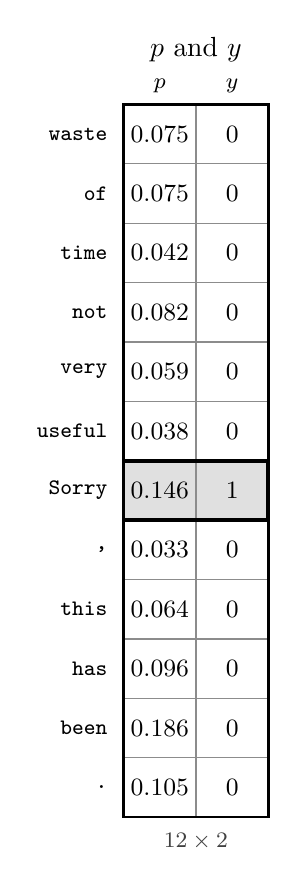
\begin{tikzpicture}
\draw[black!45, fill=white] (0.000,0.000) rectangle (0.920,-0.754);
\node[font=\small, text=black] at (0.460,-0.377) {$0.075$};
\draw[black!45, fill=white] (0.920,0.000) rectangle (1.840,-0.754);
\node[font=\small, text=black] at (1.380,-0.377) {$0$};
\draw[black!45, fill=white] (0.000,-0.754) rectangle (0.920,-1.509);
\node[font=\small, text=black] at (0.460,-1.132) {$0.075$};
\draw[black!45, fill=white] (0.920,-0.754) rectangle (1.840,-1.509);
\node[font=\small, text=black] at (1.380,-1.132) {$0$};
\draw[black!45, fill=white] (0.000,-1.509) rectangle (0.920,-2.263);
\node[font=\small, text=black] at (0.460,-1.886) {$0.042$};
\draw[black!45, fill=white] (0.920,-1.509) rectangle (1.840,-2.263);
\node[font=\small, text=black] at (1.380,-1.886) {$0$};
\draw[black!45, fill=white] (0.000,-2.263) rectangle (0.920,-3.018);
\node[font=\small, text=black] at (0.460,-2.640) {$0.082$};
\draw[black!45, fill=white] (0.920,-2.263) rectangle (1.840,-3.018);
\node[font=\small, text=black] at (1.380,-2.640) {$0$};
\draw[black!45, fill=white] (0.000,-3.018) rectangle (0.920,-3.772);
\node[font=\small, text=black] at (0.460,-3.395) {$0.059$};
\draw[black!45, fill=white] (0.920,-3.018) rectangle (1.840,-3.772);
\node[font=\small, text=black] at (1.380,-3.395) {$0$};
\draw[black!45, fill=white] (0.000,-3.772) rectangle (0.920,-4.526);
\node[font=\small, text=black] at (0.460,-4.149) {$0.038$};
\draw[black!45, fill=white] (0.920,-3.772) rectangle (1.840,-4.526);
\node[font=\small, text=black] at (1.380,-4.149) {$0$};
\draw[black!45, fill=black!12] (0.000,-4.526) rectangle (0.920,-5.281);
\node[font=\small, text=black] at (0.460,-4.904) {$0.146$};
\draw[black!45, fill=black!12] (0.920,-4.526) rectangle (1.840,-5.281);
\node[font=\small, text=black] at (1.380,-4.904) {$1$};
\draw[black!45, fill=white] (0.000,-5.281) rectangle (0.920,-6.035);
\node[font=\small, text=black] at (0.460,-5.658) {$0.033$};
\draw[black!45, fill=white] (0.920,-5.281) rectangle (1.840,-6.035);
\node[font=\small, text=black] at (1.380,-5.658) {$0$};
\draw[black!45, fill=white] (0.000,-6.035) rectangle (0.920,-6.790);
\node[font=\small, text=black] at (0.460,-6.412) {$0.064$};
\draw[black!45, fill=white] (0.920,-6.035) rectangle (1.840,-6.790);
\node[font=\small, text=black] at (1.380,-6.412) {$0$};
\draw[black!45, fill=white] (0.000,-6.790) rectangle (0.920,-7.544);
\node[font=\small, text=black] at (0.460,-7.167) {$0.096$};
\draw[black!45, fill=white] (0.920,-6.790) rectangle (1.840,-7.544);
\node[font=\small, text=black] at (1.380,-7.167) {$0$};
\draw[black!45, fill=white] (0.000,-7.544) rectangle (0.920,-8.298);
\node[font=\small, text=black] at (0.460,-7.921) {$0.186$};
\draw[black!45, fill=white] (0.920,-7.544) rectangle (1.840,-8.298);
\node[font=\small, text=black] at (1.380,-7.921) {$0$};
\draw[black!45, fill=white] (0.000,-8.298) rectangle (0.920,-9.053);
\node[font=\small, text=black] at (0.460,-8.676) {$0.105$};
\draw[black!45, fill=white] (0.920,-8.298) rectangle (1.840,-9.053);
\node[font=\small, text=black] at (1.380,-8.676) {$0$};
\draw[line width=1.4pt] (0.000,-4.526) rectangle (1.840,-5.281);
\draw[line width=0.9pt] (0.000,0.000) rectangle (1.840,-9.053);
\node[anchor=east, font=\footnotesize\ttfamily] at (-0.080,-0.377) {waste};
\node[anchor=east, font=\footnotesize\ttfamily] at (-0.080,-1.132) {of};
\node[anchor=east, font=\footnotesize\ttfamily] at (-0.080,-1.886) {time};
\node[anchor=east, font=\footnotesize\ttfamily] at (-0.080,-2.640) {not};
\node[anchor=east, font=\footnotesize\ttfamily] at (-0.080,-3.395) {very};
\node[anchor=east, font=\footnotesize\ttfamily] at (-0.080,-4.149) {useful};
\node[anchor=east, font=\footnotesize\ttfamily] at (-0.080,-4.904) {Sorry};
\node[anchor=east, font=\footnotesize\ttfamily] at (-0.080,-5.658) {{,}};
\node[anchor=east, font=\footnotesize\ttfamily] at (-0.080,-6.412) {this};
\node[anchor=east, font=\footnotesize\ttfamily] at (-0.080,-7.167) {has};
\node[anchor=east, font=\footnotesize\ttfamily] at (-0.080,-7.921) {been};
\node[anchor=east, font=\footnotesize\ttfamily] at (-0.080,-8.676) {.};
\node[anchor=south, font=\footnotesize\ttfamily] at (0.460,0.020) {$\bm{p}$};
\node[anchor=south, font=\footnotesize\ttfamily] at (1.380,0.020) {$\bm{y}$};
\node[anchor=south, font=\normalsize] at (0.920,0.420) {$\bm{p}$ and $\bm{y}$};
\node[anchor=north, font=\footnotesize, text=black!75] at (0.920,-9.133) {$12\times2$};
\end{tikzpicture}
}\\[3pt]
% AUTO-GENERATED by code/ch*_figs.py -- do not edit
{\small highlighted row (\texttt{Sorry}) $\cdot$ highlighted column ($\bm{o}_{\text{time}}$): $(1)(0.665) + (1)(0.910) + (0)(0.245) + (0)(0.090) = \mathbf{1.575}$}

\caption{Scoring every word at once. Left: the embedding table $E$ (one row per word) times \tok{time}'s
attention output, stood up as a column. Each row meets the column in a dot product; the highlighted row is
\tok{Sorry}, worked out underneath. Right: softmax turns the 12 scores $\bm{z}$ into probabilities $\bm{p}$;
next to them is the answer $\bm{y}$, a 1 on the right word and 0 everywhere else.}
\label{fig:ch8scores}
\end{figure}

\Sanity The probabilities in the column $\bm{p}$ are all positive and add to 1 (our script checks this).
\tok{Sorry} gets
\nEightPctSorry\%, second place behind \tok{\nEightTopWord}. Not great, not terrible. We need one number
for ``how bad''.

\Picture A weather forecaster says ``90\% chance of sun'' and it rains. You are very surprised, and you
trust the forecaster less. If they had said ``50--50'', the rain would surprise you a little. If they had
said ``90\% rain'', hardly at all. Surprise depends only on how much probability the forecaster put on
\emph{what actually happened}.

\Exactly The surprise of an outcome that was given probability $p$ is $-\ln p$:

\begin{center}
\small
\begin{tabular}{@{}l c c c c@{}}
\toprule
probability given to the right word & 1 & 0.5 & 0.1 & 0.01\\
surprise $-\ln p$ & \nEightSurpOne & \nEightSurpHalf & \nEightSurpTenth & \nEightSurpHundredth\\
\bottomrule
\end{tabular}
\end{center}
A certain and correct guess costs nothing. Each time the probability on the right word is divided by 10, the
surprise goes up by the same \nEightSurpTenth. For our toy, read the highlighted row of Figure~\ref{fig:ch8scores}: $\bm{y}$ points at \tok{Sorry}, where $\bm{p}$
holds \nEightPSorry, so the surprise is $-\ln \nEightPSorry = \nEightLossZero$. The other eleven cells of
$\bm{p}$ do not enter the loss at all. This number is the
\emph{loss} for this one exercise. Averaged over many exercises it is called the \emph{cross-entropy loss},
and it is the only number a language model is trained to make small:
\[
\text{loss} = -\frac{1}{N}\sum_{\text{exercises}} \ln P(\text{right next word}\mid\text{words before it}).
\]
A model that knows nothing and spreads its bets evenly over the 12 words gives each $1/12$, a loss of
$\ln 12 = \nEightUniformLoss$. Our toy, with hand-picked weights, already does a little better.

\begin{breaks}
A forecaster is judged on rain or sun. Our loss looks only at the probability on the one right word. It
does not care whether the wrong probability went to \tok{been} (close in meaning) or to \tok{.} (not close at
all). So the loss cannot tell ``nearly right'' from ``far off''; it can only tell ``put more on the right
word''.
\end{breaks}

\Why Why the logarithm and not, say, $1-p$? Chapter 1 wrote a sentence's probability as a product of
next-word probabilities. Products of many numbers below 1 collapse towards zero: a computer that multiplies
2000 probabilities of 0.5 gets exactly \nEightProdTwoThousand, because the true value is too small to store.
The log turns that product into a sum, $2000\times0.693=\nEightLogSumTwoThousand$, which is easy to store,
and a sum can be shared out exercise by exercise. The log has a second effect you should notice: as $p$
goes towards 0, $-\ln p$ grows without limit. A model that is confident \emph{and} wrong is punished far more
than one that admits it does not know. That is the behaviour we want from anything that will later say
things to customers.

\begin{wrongidea}{8.1}
\emph{``The loss is the share of wrong answers, like a test score.''} A test score only checks whether the
top answer was right. Our toy's top answer is \tok{been}, which is wrong, yet its loss of \nEightLossZero\ is
better than the \nEightUniformLoss\ of a know-nothing model, because it did put \nEightPctSorry\% on
\tok{Sorry}. The loss rewards moving probability towards the right word long before that word wins.
\end{wrongidea}

\begin{wrongidea}{8.2}
\emph{``For text, the error is the prediction minus the answer.''} It is tempting because that is how
error works when predicting a number such as a house price: $\hat y - y$. That works when both are numbers. Here the answer is the
word \tok{Sorry} and the prediction is a list of 12 probabilities: \tok{Sorry} minus \tok{been} means
nothing. What we can measure is how much probability went to the right word, and that is what surprise
measures. (Appendix A shows a nice twist: the \emph{direction} of the correction still looks like
``prediction minus answer'', one probability at a time.)
\end{wrongidea}

\begin{checkq}
A model gives the right next word a probability of 0.5. What is its loss on this exercise?
\begin{options}
\item 0.5, because half of the probability went to wrong words.
\item 0.693.
\item 0, because 0.5 is more than any other word got, so the guess was right.
\item $-0.5$, the prediction minus the answer.
\end{options}
\end{checkq}

\Summary{the loss is the surprise $-\ln p$ at the right next word, averaged over exercises, and it rewards
every bit of probability moved towards the right word.}

%---------------------------------------------------------------------
\subsection*{8.2\quad One pass, many exercises}

\Predict The full training text is \tok{waste of time Sorry , this has not been useful}: \nEightSeqLen\
tokens. How many next-word exercises does one pass through the model give us? One? Ten?

Chapter 3 built attention so that row $t$ only sees tokens $1,\ldots,t$ (the mask). So the output at every
position is an honest guess about the token after it, and all of them come out of the same pass. Running our
skeleton model once over the whole reply gives \nEightNumEx\ exercises at once:

\par\medskip\noindent\begin{minipage}{\linewidth}\centering
\fitR{% AUTO-GENERATED by code/figlib.py helpers -- do not edit
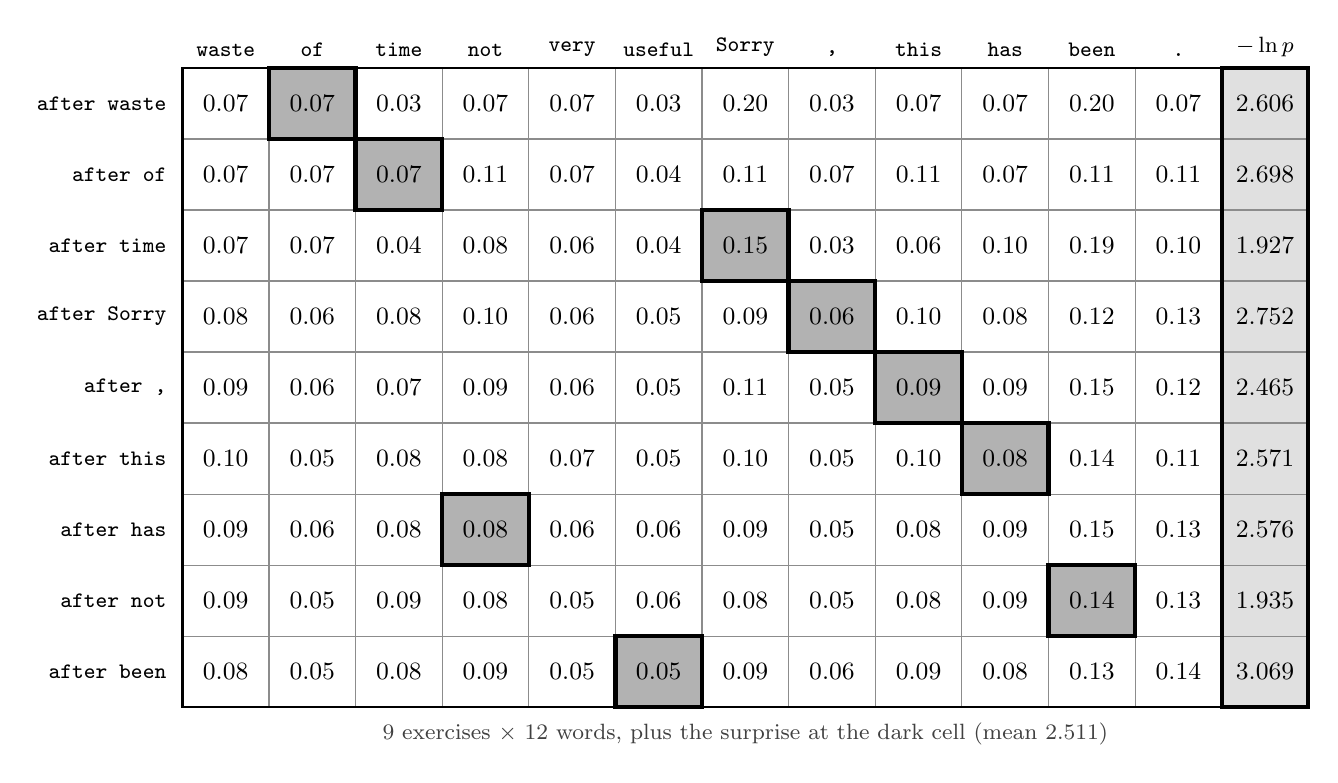
\begin{tikzpicture}
\draw[black!45, fill=white] (0.000,0.000) rectangle (1.100,-0.902);
\node[font=\small, text=black] at (0.550,-0.451) {$0.07$};
\draw[black!45, fill=black!30] (1.100,0.000) rectangle (2.200,-0.902);
\node[font=\small, text=black] at (1.650,-0.451) {$0.07$};
\draw[black!45, fill=white] (2.200,0.000) rectangle (3.300,-0.902);
\node[font=\small, text=black] at (2.750,-0.451) {$0.03$};
\draw[black!45, fill=white] (3.300,0.000) rectangle (4.400,-0.902);
\node[font=\small, text=black] at (3.850,-0.451) {$0.07$};
\draw[black!45, fill=white] (4.400,0.000) rectangle (5.500,-0.902);
\node[font=\small, text=black] at (4.950,-0.451) {$0.07$};
\draw[black!45, fill=white] (5.500,0.000) rectangle (6.600,-0.902);
\node[font=\small, text=black] at (6.050,-0.451) {$0.03$};
\draw[black!45, fill=white] (6.600,0.000) rectangle (7.700,-0.902);
\node[font=\small, text=black] at (7.150,-0.451) {$0.20$};
\draw[black!45, fill=white] (7.700,0.000) rectangle (8.800,-0.902);
\node[font=\small, text=black] at (8.250,-0.451) {$0.03$};
\draw[black!45, fill=white] (8.800,0.000) rectangle (9.900,-0.902);
\node[font=\small, text=black] at (9.350,-0.451) {$0.07$};
\draw[black!45, fill=white] (9.900,0.000) rectangle (11.000,-0.902);
\node[font=\small, text=black] at (10.450,-0.451) {$0.07$};
\draw[black!45, fill=white] (11.000,0.000) rectangle (12.100,-0.902);
\node[font=\small, text=black] at (11.550,-0.451) {$0.20$};
\draw[black!45, fill=white] (12.100,0.000) rectangle (13.200,-0.902);
\node[font=\small, text=black] at (12.650,-0.451) {$0.07$};
\draw[black!45, fill=black!12] (13.200,0.000) rectangle (14.300,-0.902);
\node[font=\small, text=black] at (13.750,-0.451) {$2.606$};
\draw[black!45, fill=white] (0.000,-0.902) rectangle (1.100,-1.804);
\node[font=\small, text=black] at (0.550,-1.353) {$0.07$};
\draw[black!45, fill=white] (1.100,-0.902) rectangle (2.200,-1.804);
\node[font=\small, text=black] at (1.650,-1.353) {$0.07$};
\draw[black!45, fill=black!30] (2.200,-0.902) rectangle (3.300,-1.804);
\node[font=\small, text=black] at (2.750,-1.353) {$0.07$};
\draw[black!45, fill=white] (3.300,-0.902) rectangle (4.400,-1.804);
\node[font=\small, text=black] at (3.850,-1.353) {$0.11$};
\draw[black!45, fill=white] (4.400,-0.902) rectangle (5.500,-1.804);
\node[font=\small, text=black] at (4.950,-1.353) {$0.07$};
\draw[black!45, fill=white] (5.500,-0.902) rectangle (6.600,-1.804);
\node[font=\small, text=black] at (6.050,-1.353) {$0.04$};
\draw[black!45, fill=white] (6.600,-0.902) rectangle (7.700,-1.804);
\node[font=\small, text=black] at (7.150,-1.353) {$0.11$};
\draw[black!45, fill=white] (7.700,-0.902) rectangle (8.800,-1.804);
\node[font=\small, text=black] at (8.250,-1.353) {$0.07$};
\draw[black!45, fill=white] (8.800,-0.902) rectangle (9.900,-1.804);
\node[font=\small, text=black] at (9.350,-1.353) {$0.11$};
\draw[black!45, fill=white] (9.900,-0.902) rectangle (11.000,-1.804);
\node[font=\small, text=black] at (10.450,-1.353) {$0.07$};
\draw[black!45, fill=white] (11.000,-0.902) rectangle (12.100,-1.804);
\node[font=\small, text=black] at (11.550,-1.353) {$0.11$};
\draw[black!45, fill=white] (12.100,-0.902) rectangle (13.200,-1.804);
\node[font=\small, text=black] at (12.650,-1.353) {$0.11$};
\draw[black!45, fill=black!12] (13.200,-0.902) rectangle (14.300,-1.804);
\node[font=\small, text=black] at (13.750,-1.353) {$2.698$};
\draw[black!45, fill=white] (0.000,-1.804) rectangle (1.100,-2.706);
\node[font=\small, text=black] at (0.550,-2.255) {$0.07$};
\draw[black!45, fill=white] (1.100,-1.804) rectangle (2.200,-2.706);
\node[font=\small, text=black] at (1.650,-2.255) {$0.07$};
\draw[black!45, fill=white] (2.200,-1.804) rectangle (3.300,-2.706);
\node[font=\small, text=black] at (2.750,-2.255) {$0.04$};
\draw[black!45, fill=white] (3.300,-1.804) rectangle (4.400,-2.706);
\node[font=\small, text=black] at (3.850,-2.255) {$0.08$};
\draw[black!45, fill=white] (4.400,-1.804) rectangle (5.500,-2.706);
\node[font=\small, text=black] at (4.950,-2.255) {$0.06$};
\draw[black!45, fill=white] (5.500,-1.804) rectangle (6.600,-2.706);
\node[font=\small, text=black] at (6.050,-2.255) {$0.04$};
\draw[black!45, fill=black!30] (6.600,-1.804) rectangle (7.700,-2.706);
\node[font=\small, text=black] at (7.150,-2.255) {$0.15$};
\draw[black!45, fill=white] (7.700,-1.804) rectangle (8.800,-2.706);
\node[font=\small, text=black] at (8.250,-2.255) {$0.03$};
\draw[black!45, fill=white] (8.800,-1.804) rectangle (9.900,-2.706);
\node[font=\small, text=black] at (9.350,-2.255) {$0.06$};
\draw[black!45, fill=white] (9.900,-1.804) rectangle (11.000,-2.706);
\node[font=\small, text=black] at (10.450,-2.255) {$0.10$};
\draw[black!45, fill=white] (11.000,-1.804) rectangle (12.100,-2.706);
\node[font=\small, text=black] at (11.550,-2.255) {$0.19$};
\draw[black!45, fill=white] (12.100,-1.804) rectangle (13.200,-2.706);
\node[font=\small, text=black] at (12.650,-2.255) {$0.10$};
\draw[black!45, fill=black!12] (13.200,-1.804) rectangle (14.300,-2.706);
\node[font=\small, text=black] at (13.750,-2.255) {$1.927$};
\draw[black!45, fill=white] (0.000,-2.706) rectangle (1.100,-3.608);
\node[font=\small, text=black] at (0.550,-3.157) {$0.08$};
\draw[black!45, fill=white] (1.100,-2.706) rectangle (2.200,-3.608);
\node[font=\small, text=black] at (1.650,-3.157) {$0.06$};
\draw[black!45, fill=white] (2.200,-2.706) rectangle (3.300,-3.608);
\node[font=\small, text=black] at (2.750,-3.157) {$0.08$};
\draw[black!45, fill=white] (3.300,-2.706) rectangle (4.400,-3.608);
\node[font=\small, text=black] at (3.850,-3.157) {$0.10$};
\draw[black!45, fill=white] (4.400,-2.706) rectangle (5.500,-3.608);
\node[font=\small, text=black] at (4.950,-3.157) {$0.06$};
\draw[black!45, fill=white] (5.500,-2.706) rectangle (6.600,-3.608);
\node[font=\small, text=black] at (6.050,-3.157) {$0.05$};
\draw[black!45, fill=white] (6.600,-2.706) rectangle (7.700,-3.608);
\node[font=\small, text=black] at (7.150,-3.157) {$0.09$};
\draw[black!45, fill=black!30] (7.700,-2.706) rectangle (8.800,-3.608);
\node[font=\small, text=black] at (8.250,-3.157) {$0.06$};
\draw[black!45, fill=white] (8.800,-2.706) rectangle (9.900,-3.608);
\node[font=\small, text=black] at (9.350,-3.157) {$0.10$};
\draw[black!45, fill=white] (9.900,-2.706) rectangle (11.000,-3.608);
\node[font=\small, text=black] at (10.450,-3.157) {$0.08$};
\draw[black!45, fill=white] (11.000,-2.706) rectangle (12.100,-3.608);
\node[font=\small, text=black] at (11.550,-3.157) {$0.12$};
\draw[black!45, fill=white] (12.100,-2.706) rectangle (13.200,-3.608);
\node[font=\small, text=black] at (12.650,-3.157) {$0.13$};
\draw[black!45, fill=black!12] (13.200,-2.706) rectangle (14.300,-3.608);
\node[font=\small, text=black] at (13.750,-3.157) {$2.752$};
\draw[black!45, fill=white] (0.000,-3.608) rectangle (1.100,-4.510);
\node[font=\small, text=black] at (0.550,-4.059) {$0.09$};
\draw[black!45, fill=white] (1.100,-3.608) rectangle (2.200,-4.510);
\node[font=\small, text=black] at (1.650,-4.059) {$0.06$};
\draw[black!45, fill=white] (2.200,-3.608) rectangle (3.300,-4.510);
\node[font=\small, text=black] at (2.750,-4.059) {$0.07$};
\draw[black!45, fill=white] (3.300,-3.608) rectangle (4.400,-4.510);
\node[font=\small, text=black] at (3.850,-4.059) {$0.09$};
\draw[black!45, fill=white] (4.400,-3.608) rectangle (5.500,-4.510);
\node[font=\small, text=black] at (4.950,-4.059) {$0.06$};
\draw[black!45, fill=white] (5.500,-3.608) rectangle (6.600,-4.510);
\node[font=\small, text=black] at (6.050,-4.059) {$0.05$};
\draw[black!45, fill=white] (6.600,-3.608) rectangle (7.700,-4.510);
\node[font=\small, text=black] at (7.150,-4.059) {$0.11$};
\draw[black!45, fill=white] (7.700,-3.608) rectangle (8.800,-4.510);
\node[font=\small, text=black] at (8.250,-4.059) {$0.05$};
\draw[black!45, fill=black!30] (8.800,-3.608) rectangle (9.900,-4.510);
\node[font=\small, text=black] at (9.350,-4.059) {$0.09$};
\draw[black!45, fill=white] (9.900,-3.608) rectangle (11.000,-4.510);
\node[font=\small, text=black] at (10.450,-4.059) {$0.09$};
\draw[black!45, fill=white] (11.000,-3.608) rectangle (12.100,-4.510);
\node[font=\small, text=black] at (11.550,-4.059) {$0.15$};
\draw[black!45, fill=white] (12.100,-3.608) rectangle (13.200,-4.510);
\node[font=\small, text=black] at (12.650,-4.059) {$0.12$};
\draw[black!45, fill=black!12] (13.200,-3.608) rectangle (14.300,-4.510);
\node[font=\small, text=black] at (13.750,-4.059) {$2.465$};
\draw[black!45, fill=white] (0.000,-4.510) rectangle (1.100,-5.412);
\node[font=\small, text=black] at (0.550,-4.961) {$0.10$};
\draw[black!45, fill=white] (1.100,-4.510) rectangle (2.200,-5.412);
\node[font=\small, text=black] at (1.650,-4.961) {$0.05$};
\draw[black!45, fill=white] (2.200,-4.510) rectangle (3.300,-5.412);
\node[font=\small, text=black] at (2.750,-4.961) {$0.08$};
\draw[black!45, fill=white] (3.300,-4.510) rectangle (4.400,-5.412);
\node[font=\small, text=black] at (3.850,-4.961) {$0.08$};
\draw[black!45, fill=white] (4.400,-4.510) rectangle (5.500,-5.412);
\node[font=\small, text=black] at (4.950,-4.961) {$0.07$};
\draw[black!45, fill=white] (5.500,-4.510) rectangle (6.600,-5.412);
\node[font=\small, text=black] at (6.050,-4.961) {$0.05$};
\draw[black!45, fill=white] (6.600,-4.510) rectangle (7.700,-5.412);
\node[font=\small, text=black] at (7.150,-4.961) {$0.10$};
\draw[black!45, fill=white] (7.700,-4.510) rectangle (8.800,-5.412);
\node[font=\small, text=black] at (8.250,-4.961) {$0.05$};
\draw[black!45, fill=white] (8.800,-4.510) rectangle (9.900,-5.412);
\node[font=\small, text=black] at (9.350,-4.961) {$0.10$};
\draw[black!45, fill=black!30] (9.900,-4.510) rectangle (11.000,-5.412);
\node[font=\small, text=black] at (10.450,-4.961) {$0.08$};
\draw[black!45, fill=white] (11.000,-4.510) rectangle (12.100,-5.412);
\node[font=\small, text=black] at (11.550,-4.961) {$0.14$};
\draw[black!45, fill=white] (12.100,-4.510) rectangle (13.200,-5.412);
\node[font=\small, text=black] at (12.650,-4.961) {$0.11$};
\draw[black!45, fill=black!12] (13.200,-4.510) rectangle (14.300,-5.412);
\node[font=\small, text=black] at (13.750,-4.961) {$2.571$};
\draw[black!45, fill=white] (0.000,-5.412) rectangle (1.100,-6.314);
\node[font=\small, text=black] at (0.550,-5.863) {$0.09$};
\draw[black!45, fill=white] (1.100,-5.412) rectangle (2.200,-6.314);
\node[font=\small, text=black] at (1.650,-5.863) {$0.06$};
\draw[black!45, fill=white] (2.200,-5.412) rectangle (3.300,-6.314);
\node[font=\small, text=black] at (2.750,-5.863) {$0.08$};
\draw[black!45, fill=black!30] (3.300,-5.412) rectangle (4.400,-6.314);
\node[font=\small, text=black] at (3.850,-5.863) {$0.08$};
\draw[black!45, fill=white] (4.400,-5.412) rectangle (5.500,-6.314);
\node[font=\small, text=black] at (4.950,-5.863) {$0.06$};
\draw[black!45, fill=white] (5.500,-5.412) rectangle (6.600,-6.314);
\node[font=\small, text=black] at (6.050,-5.863) {$0.06$};
\draw[black!45, fill=white] (6.600,-5.412) rectangle (7.700,-6.314);
\node[font=\small, text=black] at (7.150,-5.863) {$0.09$};
\draw[black!45, fill=white] (7.700,-5.412) rectangle (8.800,-6.314);
\node[font=\small, text=black] at (8.250,-5.863) {$0.05$};
\draw[black!45, fill=white] (8.800,-5.412) rectangle (9.900,-6.314);
\node[font=\small, text=black] at (9.350,-5.863) {$0.08$};
\draw[black!45, fill=white] (9.900,-5.412) rectangle (11.000,-6.314);
\node[font=\small, text=black] at (10.450,-5.863) {$0.09$};
\draw[black!45, fill=white] (11.000,-5.412) rectangle (12.100,-6.314);
\node[font=\small, text=black] at (11.550,-5.863) {$0.15$};
\draw[black!45, fill=white] (12.100,-5.412) rectangle (13.200,-6.314);
\node[font=\small, text=black] at (12.650,-5.863) {$0.13$};
\draw[black!45, fill=black!12] (13.200,-5.412) rectangle (14.300,-6.314);
\node[font=\small, text=black] at (13.750,-5.863) {$2.576$};
\draw[black!45, fill=white] (0.000,-6.314) rectangle (1.100,-7.216);
\node[font=\small, text=black] at (0.550,-6.765) {$0.09$};
\draw[black!45, fill=white] (1.100,-6.314) rectangle (2.200,-7.216);
\node[font=\small, text=black] at (1.650,-6.765) {$0.05$};
\draw[black!45, fill=white] (2.200,-6.314) rectangle (3.300,-7.216);
\node[font=\small, text=black] at (2.750,-6.765) {$0.09$};
\draw[black!45, fill=white] (3.300,-6.314) rectangle (4.400,-7.216);
\node[font=\small, text=black] at (3.850,-6.765) {$0.08$};
\draw[black!45, fill=white] (4.400,-6.314) rectangle (5.500,-7.216);
\node[font=\small, text=black] at (4.950,-6.765) {$0.05$};
\draw[black!45, fill=white] (5.500,-6.314) rectangle (6.600,-7.216);
\node[font=\small, text=black] at (6.050,-6.765) {$0.06$};
\draw[black!45, fill=white] (6.600,-6.314) rectangle (7.700,-7.216);
\node[font=\small, text=black] at (7.150,-6.765) {$0.08$};
\draw[black!45, fill=white] (7.700,-6.314) rectangle (8.800,-7.216);
\node[font=\small, text=black] at (8.250,-6.765) {$0.05$};
\draw[black!45, fill=white] (8.800,-6.314) rectangle (9.900,-7.216);
\node[font=\small, text=black] at (9.350,-6.765) {$0.08$};
\draw[black!45, fill=white] (9.900,-6.314) rectangle (11.000,-7.216);
\node[font=\small, text=black] at (10.450,-6.765) {$0.09$};
\draw[black!45, fill=black!30] (11.000,-6.314) rectangle (12.100,-7.216);
\node[font=\small, text=black] at (11.550,-6.765) {$0.14$};
\draw[black!45, fill=white] (12.100,-6.314) rectangle (13.200,-7.216);
\node[font=\small, text=black] at (12.650,-6.765) {$0.13$};
\draw[black!45, fill=black!12] (13.200,-6.314) rectangle (14.300,-7.216);
\node[font=\small, text=black] at (13.750,-6.765) {$1.935$};
\draw[black!45, fill=white] (0.000,-7.216) rectangle (1.100,-8.118);
\node[font=\small, text=black] at (0.550,-7.667) {$0.08$};
\draw[black!45, fill=white] (1.100,-7.216) rectangle (2.200,-8.118);
\node[font=\small, text=black] at (1.650,-7.667) {$0.05$};
\draw[black!45, fill=white] (2.200,-7.216) rectangle (3.300,-8.118);
\node[font=\small, text=black] at (2.750,-7.667) {$0.08$};
\draw[black!45, fill=white] (3.300,-7.216) rectangle (4.400,-8.118);
\node[font=\small, text=black] at (3.850,-7.667) {$0.09$};
\draw[black!45, fill=white] (4.400,-7.216) rectangle (5.500,-8.118);
\node[font=\small, text=black] at (4.950,-7.667) {$0.05$};
\draw[black!45, fill=black!30] (5.500,-7.216) rectangle (6.600,-8.118);
\node[font=\small, text=black] at (6.050,-7.667) {$0.05$};
\draw[black!45, fill=white] (6.600,-7.216) rectangle (7.700,-8.118);
\node[font=\small, text=black] at (7.150,-7.667) {$0.09$};
\draw[black!45, fill=white] (7.700,-7.216) rectangle (8.800,-8.118);
\node[font=\small, text=black] at (8.250,-7.667) {$0.06$};
\draw[black!45, fill=white] (8.800,-7.216) rectangle (9.900,-8.118);
\node[font=\small, text=black] at (9.350,-7.667) {$0.09$};
\draw[black!45, fill=white] (9.900,-7.216) rectangle (11.000,-8.118);
\node[font=\small, text=black] at (10.450,-7.667) {$0.08$};
\draw[black!45, fill=white] (11.000,-7.216) rectangle (12.100,-8.118);
\node[font=\small, text=black] at (11.550,-7.667) {$0.13$};
\draw[black!45, fill=white] (12.100,-7.216) rectangle (13.200,-8.118);
\node[font=\small, text=black] at (12.650,-7.667) {$0.14$};
\draw[black!45, fill=black!12] (13.200,-7.216) rectangle (14.300,-8.118);
\node[font=\small, text=black] at (13.750,-7.667) {$3.069$};
\draw[line width=1.4pt] (13.200,0.000) rectangle (14.300,-8.118);
\draw[line width=1.6pt] (1.100,0.000) rectangle (2.200,-0.902);
\draw[line width=1.6pt] (2.200,-0.902) rectangle (3.300,-1.804);
\draw[line width=1.6pt] (6.600,-1.804) rectangle (7.700,-2.706);
\draw[line width=1.6pt] (7.700,-2.706) rectangle (8.800,-3.608);
\draw[line width=1.6pt] (8.800,-3.608) rectangle (9.900,-4.510);
\draw[line width=1.6pt] (9.900,-4.510) rectangle (11.000,-5.412);
\draw[line width=1.6pt] (3.300,-5.412) rectangle (4.400,-6.314);
\draw[line width=1.6pt] (11.000,-6.314) rectangle (12.100,-7.216);
\draw[line width=1.6pt] (5.500,-7.216) rectangle (6.600,-8.118);
\draw[line width=0.9pt] (0.000,0.000) rectangle (14.300,-8.118);
\node[anchor=east, font=\footnotesize\ttfamily] at (-0.080,-0.451) {after \texttt{waste}};
\node[anchor=east, font=\footnotesize\ttfamily] at (-0.080,-1.353) {after \texttt{of}};
\node[anchor=east, font=\footnotesize\ttfamily] at (-0.080,-2.255) {after \texttt{time}};
\node[anchor=east, font=\footnotesize\ttfamily] at (-0.080,-3.157) {after \texttt{Sorry}};
\node[anchor=east, font=\footnotesize\ttfamily] at (-0.080,-4.059) {after \texttt{{,}}};
\node[anchor=east, font=\footnotesize\ttfamily] at (-0.080,-4.961) {after \texttt{this}};
\node[anchor=east, font=\footnotesize\ttfamily] at (-0.080,-5.863) {after \texttt{has}};
\node[anchor=east, font=\footnotesize\ttfamily] at (-0.080,-6.765) {after \texttt{not}};
\node[anchor=east, font=\footnotesize\ttfamily] at (-0.080,-7.667) {after \texttt{been}};
\node[anchor=south, font=\footnotesize\ttfamily] at (0.550,0.020) {\texttt{waste}};
\node[anchor=south, font=\footnotesize\ttfamily] at (1.650,0.020) {\texttt{of}};
\node[anchor=south, font=\footnotesize\ttfamily] at (2.750,0.020) {\texttt{time}};
\node[anchor=south, font=\footnotesize\ttfamily] at (3.850,0.020) {\texttt{not}};
\node[anchor=south, font=\footnotesize\ttfamily] at (4.950,0.020) {\texttt{very}};
\node[anchor=south, font=\footnotesize\ttfamily] at (6.050,0.020) {\texttt{useful}};
\node[anchor=south, font=\footnotesize\ttfamily] at (7.150,0.020) {\texttt{Sorry}};
\node[anchor=south, font=\footnotesize\ttfamily] at (8.250,0.020) {\texttt{{,}}};
\node[anchor=south, font=\footnotesize\ttfamily] at (9.350,0.020) {\texttt{this}};
\node[anchor=south, font=\footnotesize\ttfamily] at (10.450,0.020) {\texttt{has}};
\node[anchor=south, font=\footnotesize\ttfamily] at (11.550,0.020) {\texttt{been}};
\node[anchor=south, font=\footnotesize\ttfamily] at (12.650,0.020) {\texttt{.}};
\node[anchor=south, font=\footnotesize\ttfamily] at (13.750,0.020) {$-\ln p$};
\node[anchor=north, font=\footnotesize, text=black!75] at (7.150,-8.198) {9 exercises $\times$ 12 words, plus the surprise at the dark cell (mean 2.511)};
\end{tikzpicture}
}
\captionof{figure}{One pass, nine exercises. Each row is the toy's probability for every next word after reading up
to the word on the left; the dark cell is the probability it gave the word that really came next. The column on
the right is the surprise $-\ln p$ for that dark cell. Row 3 (after \tok{time}) is the exercise of \S8.1.}
\end{minipage}\par\medskip

The average surprise over the nine is \nEightMeanLoss; the sum is \nEightSumLoss. Look at row 3, after
\tok{time}: it is the
same \nEightLossZero\ as in \S8.1, to every decimal, even though the model now also saw the six reply words.
That is the mask doing its job (our script asserts the two are equal).

\Picture A tutor marks a student's essay line by line. Before the student writes line 4, the tutor shows the
correct line 3, so one early slip does not ruin every later line. In training, the model is always given the
true earlier words, never its own guesses. This is called \emph{teacher forcing} (Williams and Zipser, 1989).

\begin{breaks}
The tutor helps during practice only. When the model writes a real reply (Chapter 7), nobody hands it the
correct earlier words; it builds on its own. This gap between practice and use is one source of the
compounding errors we called hallucination in Chapter 1.
\end{breaks}

\Why Without the mask, each pass would give one honest exercise and the rest would be spoiled by peeking.
With it, every position of every sentence in a batch is an exercise. Here is the smallest batch that
shows it: two replies of three tokens each, stacked as in \S3.9, and the grid of words they must guess.

\par\medskip\noindent\begin{minipage}{\linewidth}\centering
\fitR{% AUTO-GENERATED by code/figlib.py helpers -- do not edit
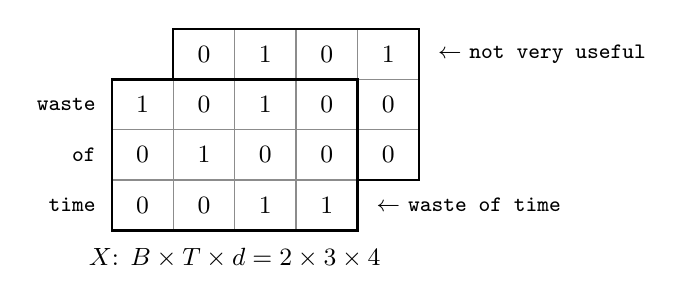
\begin{tikzpicture}
\fill[white] (0.780,0.640) rectangle (3.900,-1.279);
\draw[black!45, fill=white] (0.780,0.640) rectangle (1.560,0.000);
\node[font=\small, text=black] at (1.170,0.320) {$0$};
\draw[black!45, fill=white] (1.560,0.640) rectangle (2.340,0.000);
\node[font=\small, text=black] at (1.950,0.320) {$1$};
\draw[black!45, fill=white] (2.340,0.640) rectangle (3.120,0.000);
\node[font=\small, text=black] at (2.730,0.320) {$0$};
\draw[black!45, fill=white] (3.120,0.640) rectangle (3.900,0.000);
\node[font=\small, text=black] at (3.510,0.320) {$1$};
\draw[black!45, fill=white] (0.780,0.000) rectangle (1.560,-0.640);
\node[font=\small, text=black] at (1.170,-0.320) {$1$};
\draw[black!45, fill=white] (1.560,0.000) rectangle (2.340,-0.640);
\node[font=\small, text=black] at (1.950,-0.320) {$0$};
\draw[black!45, fill=white] (2.340,0.000) rectangle (3.120,-0.640);
\node[font=\small, text=black] at (2.730,-0.320) {$0$};
\draw[black!45, fill=white] (3.120,0.000) rectangle (3.900,-0.640);
\node[font=\small, text=black] at (3.510,-0.320) {$0$};
\draw[black!45, fill=white] (0.780,-0.640) rectangle (1.560,-1.279);
\node[font=\small, text=black] at (1.170,-0.959) {$0$};
\draw[black!45, fill=white] (1.560,-0.640) rectangle (2.340,-1.279);
\node[font=\small, text=black] at (1.950,-0.959) {$0$};
\draw[black!45, fill=white] (2.340,-0.640) rectangle (3.120,-1.279);
\node[font=\small, text=black] at (2.730,-0.959) {$1$};
\draw[black!45, fill=white] (3.120,-0.640) rectangle (3.900,-1.279);
\node[font=\small, text=black] at (3.510,-0.959) {$0$};
\draw[line width=0.9pt] (0.780,0.640) rectangle (3.900,-1.279);
\node[anchor=west, font=\footnotesize] at (4.020,0.320) {$\leftarrow$ \texttt{not very useful}};
\fill[white] (0.000,0.000) rectangle (3.120,-1.919);
\draw[black!45, fill=white] (0.000,0.000) rectangle (0.780,-0.640);
\node[font=\small, text=black] at (0.390,-0.320) {$1$};
\draw[black!45, fill=white] (0.780,0.000) rectangle (1.560,-0.640);
\node[font=\small, text=black] at (1.170,-0.320) {$0$};
\draw[black!45, fill=white] (1.560,0.000) rectangle (2.340,-0.640);
\node[font=\small, text=black] at (1.950,-0.320) {$1$};
\draw[black!45, fill=white] (2.340,0.000) rectangle (3.120,-0.640);
\node[font=\small, text=black] at (2.730,-0.320) {$0$};
\draw[black!45, fill=white] (0.000,-0.640) rectangle (0.780,-1.279);
\node[font=\small, text=black] at (0.390,-0.959) {$0$};
\draw[black!45, fill=white] (0.780,-0.640) rectangle (1.560,-1.279);
\node[font=\small, text=black] at (1.170,-0.959) {$1$};
\draw[black!45, fill=white] (1.560,-0.640) rectangle (2.340,-1.279);
\node[font=\small, text=black] at (1.950,-0.959) {$0$};
\draw[black!45, fill=white] (2.340,-0.640) rectangle (3.120,-1.279);
\node[font=\small, text=black] at (2.730,-0.959) {$0$};
\draw[black!45, fill=white] (0.000,-1.279) rectangle (0.780,-1.919);
\node[font=\small, text=black] at (0.390,-1.599) {$0$};
\draw[black!45, fill=white] (0.780,-1.279) rectangle (1.560,-1.919);
\node[font=\small, text=black] at (1.170,-1.599) {$0$};
\draw[black!45, fill=white] (1.560,-1.279) rectangle (2.340,-1.919);
\node[font=\small, text=black] at (1.950,-1.599) {$1$};
\draw[black!45, fill=white] (2.340,-1.279) rectangle (3.120,-1.919);
\node[font=\small, text=black] at (2.730,-1.599) {$1$};
\draw[line width=0.9pt] (0.000,0.000) rectangle (3.120,-1.919);
\node[anchor=east, font=\footnotesize\ttfamily] at (-0.080,-0.320) {waste};
\node[anchor=east, font=\footnotesize\ttfamily] at (-0.080,-0.959) {of};
\node[anchor=east, font=\footnotesize\ttfamily] at (-0.080,-1.599) {time};
\node[anchor=west, font=\footnotesize] at (3.240,-1.599) {$\leftarrow$ \texttt{waste of time}};
\node[anchor=north, font=\small] at (1.560,-2.019) {$X$: $B\times T\times d = 2\times3\times4$};
\end{tikzpicture}
\qquad
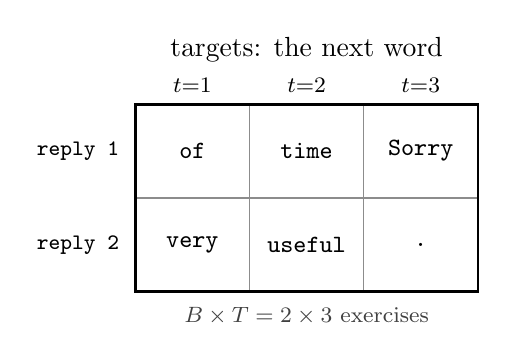
\begin{tikzpicture}
\draw[black!45, fill=white] (0.000,0.000) rectangle (1.450,-1.189);
\node[font=\small, text=black] at (0.725,-0.594) {\texttt{of}};
\draw[black!45, fill=white] (1.450,0.000) rectangle (2.900,-1.189);
\node[font=\small, text=black] at (2.175,-0.594) {\texttt{time}};
\draw[black!45, fill=white] (2.900,0.000) rectangle (4.350,-1.189);
\node[font=\small, text=black] at (3.625,-0.594) {\texttt{Sorry}};
\draw[black!45, fill=white] (0.000,-1.189) rectangle (1.450,-2.378);
\node[font=\small, text=black] at (0.725,-1.783) {\texttt{very}};
\draw[black!45, fill=white] (1.450,-1.189) rectangle (2.900,-2.378);
\node[font=\small, text=black] at (2.175,-1.783) {\texttt{useful}};
\draw[black!45, fill=white] (2.900,-1.189) rectangle (4.350,-2.378);
\node[font=\small, text=black] at (3.625,-1.783) {\texttt{.}};
\draw[line width=0.9pt] (0.000,0.000) rectangle (4.350,-2.378);
\node[anchor=east, font=\footnotesize\ttfamily] at (-0.080,-0.594) {reply 1};
\node[anchor=east, font=\footnotesize\ttfamily] at (-0.080,-1.783) {reply 2};
\node[anchor=south, font=\footnotesize\ttfamily] at (0.725,0.020) {$t{=}1$};
\node[anchor=south, font=\footnotesize\ttfamily] at (2.175,0.020) {$t{=}2$};
\node[anchor=south, font=\footnotesize\ttfamily] at (3.625,0.020) {$t{=}3$};
\node[anchor=south, font=\normalsize] at (2.175,0.420) {targets: the next word};
\node[anchor=north, font=\footnotesize, text=black!75] at (2.175,-2.458) {$B\times T = 2\times3$ exercises};
\end{tikzpicture}
}
\captionof{figure}{A batch of $B=2$ replies, $T=3$ tokens each. Left: the input arrows, one $3\times4$ sheet per reply,
stacked into a $2\times3\times4$ block. Right: the targets, each input shifted one place to the left, so every
cell is one exercise. (The full stop that ends reply 2 is our assumption, for the example.)}
\end{minipage}\par\medskip

A real batch of 32 sequences of 64 tokens is the same picture, bigger: $32\times64$ exercises per pass. That factor, more than
anything clever, is why transformers can be trained on so much text.

\begin{wrongidea}{8.5}
\emph{``A sentence gives the model one exercise.''} It is tempting because the model writes one token at a
time. That is true when the model \emph{writes}. When it \emph{learns},
every position is an exercise, all solved together in one pass. The figure in \S8.2 has nine.
\end{wrongidea}

\begin{checkq}
In the figure of \S8.2, why is the probability of \tok{Sorry} in row 3 exactly the same as when the model saw only
\tok{waste of time}?
\begin{options}
\item Because \tok{Sorry} is the most likely word in both cases.
\item Because the mask stops row 3 from seeing any later token, so the later words cannot change it.
\item Because the model has not been trained yet.
\item Because each sentence gives only one exercise, so row 3 is computed alone.
\end{options}
\end{checkq}

\Summary{thanks to the mask, one pass over $T$ tokens gives $T-1$ honest exercises, and the loss is their
average surprise.}

%---------------------------------------------------------------------
\subsection*{8.3\quad The landscape, and walking downhill}

\Predict Keep everything in the toy fixed except one knob: the direction of \tok{time}'s query. At the
moment it points straight at \tok{waste}'s key (angle $0^\circ$, as in \S3.6). Suppose we turned it to point
at \tok{of}'s key instead ($90^\circ$). Will the loss go up or down? By roughly how much?

\Picture You are on a hillside in thick fog, and you want to reach the lowest point of the valley. You cannot
see it. What you can do is feel the ground: put one foot a little to the left, then a little to the right,
and notice which way is lower. Step that way. Repeat. As an algorithm: look at where you stand, find which way is downhill, take a
step, repeat. Here the hillside is the loss, and your position is the
setting of the knob.

Let us draw the hillside for our one knob. We turn \tok{time}'s query through every angle, keeping its length
at \lenQ, and compute the loss each time:

\par\medskip\noindent\begin{minipage}{\linewidth}\centering
\begin{tikzpicture}
\begin{axis}[width=12.5cm, height=5.4cm, xmin=-120, xmax=180, ymin=1.8, ymax=2.85,
  xlabel={angle of \texttt{time}'s query from \texttt{waste}'s key (degrees)}, ylabel={loss},
  label style={font=\small}, tick label style={font=\footnotesize}, axis lines*=left,
  xtick={-90,-45,0,45,90,135,180}]
\addplot[black, thick, no marks] table[x=theta, y=loss] {data_ch8/landscape.dat};
\addplot[black!55, only marks, mark=*, mark size=1.6pt] table[x=theta, y=loss] {data_ch8/pathSmall.dat};
\addplot[black, only marks, mark=square*, mark size=1.7pt] table[x=theta, y=loss] {data_ch8/pathGood.dat};
\addplot[black!70, only marks, mark=triangle*, mark size=2.4pt] table[x=theta, y=loss] {data_ch8/pathBig.dat};
\node[font=\footnotesize, anchor=west] at (axis cs:94,2.42) {start};
\node[font=\footnotesize, anchor=north] at (axis cs:\nEightThetaMin,1.9) {bottom: \nEightThetaMin$^\circ$};
\node[font=\footnotesize, align=left, anchor=north west] at (axis cs:-115,2.84) {circles: small steps\\squares: good steps\\triangles: steps too big};
\end{axis}
\end{tikzpicture}
\captionof{figure}{A real slice of the toy's loss landscape: one knob, the direction of \tok{time}'s query. Marks show
15 steps of three walkers who all start at $90^\circ$ and differ only in step size.}
\end{minipage}\par\medskip

\Sanity At $90^\circ$ (pointing at \tok{of}) the loss is \nEightLossAtNinety; at $0^\circ$ (pointing at
\tok{waste}, our hand-picked setting) it is \nEightLossAtZero; the very bottom is at \nEightThetaMin$^\circ$,
with loss \nEightLossAtMin. So the hand-picked direction was nearly the best one, and pointing at \tok{of}
is worse. Does that match your prediction?

Now be the walker in the fog at $90^\circ$. Probe: at $89^\circ$ the loss is \nEightProbeLeft, at
$91^\circ$ it is \nEightProbeRight. Lower is towards smaller angles, so turn towards \tok{waste}. The
steepness is about \nEightSlopeNinety\ loss per degree. How far to step? The rule every training method uses
is
\[
\text{new setting} = \text{old setting} - (\text{step size}) \times (\text{slope}).
\]
The step size is called the \emph{learning rate}. Three walkers, three learning rates, 15 steps each:
\begin{itemize}
\item \textbf{Small} (\nEightLrSmall): after 15 steps the angle has crawled from $90^\circ$ to only
\nEightThetaSmallEnd$^\circ$. Safe and painfully slow.
\item \textbf{Good} (\nEightLrGood, ten times larger): the first step alone moves to
\nEightGoodFirst$^\circ$; after 15 steps it is at \nEightThetaGoodEnd$^\circ$, close to the bottom. Steps
shrink by themselves near the bottom, because the ground flattens there and the slope gets small.
\item \textbf{Too big} (\nEightLrBig, fifty times the small one): the first step overshoots the valley to
\nEightBigFirst$^\circ$, the next jumps back to \nEightBigSecond$^\circ$, then \nEightBigThird$^\circ$,
\nEightBigFourth$^\circ$, and so on. It bounces between the two sides of the valley forever and ends at
loss \nEightLossBigEnd, worse than where the good walker is.
\end{itemize}

\Exactly A real model has not one knob but millions (every number in every $W$). The slope of the loss for
every knob at once is called the \emph{gradient}, an arrow in knob-space that points uphill. Gradient
descent steps against it: $\bm{\theta}\leftarrow\bm{\theta}-\eta\,\bm{g}$, where $\bm{\theta}$ lists every
knob, $\eta$ is the learning rate and $\bm{g}$ is the gradient. The idea has been around since Cauchy (1847).

\begin{breaks}
Our probe-left-probe-right trick needs two extra passes per knob. With millions of knobs that is hopeless.
Real training gets all the slopes at once, for the price of about one extra pass, with an exact
bookkeeping method called \emph{backpropagation} (Rumelhart, Hinton and Williams, 1986). Appendix A works it
out and checks every result against probing. The picture of a hill also hides how strange a landscape with
millions of directions is: there are many valleys, and wide flat regions.
\end{breaks}

\Why Why not jump straight to the bottom? Because nobody has a formula for where it is. All we can ever know
is the ground under our feet: the loss and its slope at the current setting. Small, repeated, local
corrections is the only plan that works without a map, which is why every model in this book is trained this
way.

\begin{wrongidea}{8.3}
\emph{``A bigger step size always learns faster.''} It is tempting because a bigger step covers more ground. The
triangles show the opposite: with the larger step the walker bounces from one side of the valley to the other and never settles, ending higher than the good walker. Too large a step overshoots the valley; past a point it bounces or flies off. Choosing the learning rate is
one of the first decisions in any training run (Chapter 11).
\end{wrongidea}

\begin{wrongidea}{8.7}
\emph{``Training finds the best possible weights.''} Our one-knob slice has a single valley, so here it
does. A real landscape has many valleys, and walking downhill finds a low one near where you started, not the
lowest one on the map. In practice that turns out to be good enough, and nobody can check that it is the best.
\end{wrongidea}

\begin{checkq}
You probe a knob and find the loss is 3.10 a little to the left and 3.02 a little to the right. With a
sensible learning rate, what do you do?
\begin{options}
\item Step left, because the loss there is bigger and you want a bigger change.
\item Step right by a small amount in proportion to the slope.
\item Step right as far as possible, since bigger steps learn faster.
\item Stop: you have found the best setting, since one side is lower.
\end{options}
\end{checkq}

\Summary{the loss draws a landscape over the knobs; training probes the slope where it stands and takes a
step downhill whose size, the learning rate, must be neither too small nor too large.}

%---------------------------------------------------------------------
\subsection*{8.4\quad The payoff: watching the arrows turn}

\Predict In \S3.10 we promised that training turns \tok{time}'s query towards \tok{waste}'s key and
stretches it. Let us test that honestly. Throw away our hand-picked $W_Q$, $W_K$, $W_V$ and start from random
numbers. At the start, \tok{time} gives \tok{waste} a share of \nEightTrainShareStart, and its query points
\nEightTrainAngStart$^\circ$ away from \tok{waste}'s key. After 60 downhill steps on the single exercise
``\tok{waste of time} $\to$ \tok{Sorry}'', what do you expect the share and the angle to be?

We train all three machines at once, starting from the same random numbers, with three learning rates. Here
the slopes come from backpropagation, the method of Appendix A.

\par\medskip\noindent\begin{minipage}{\linewidth}\centering
\begin{tikzpicture}
\begin{axis}[width=7.4cm, height=4.6cm, xmin=0, xmax=60, ymin=0, ymax=1.05, xlabel={step},
  ylabel={share of attention on \texttt{waste}}, label style={font=\small}, tick label style={font=\footnotesize},
  axis lines*=left]
\addplot[black!55, thick, no marks] table[x=step, y=share] {data_ch8/toySlow.dat};
\addplot[black, very thick, no marks] table[x=step, y=share] {data_ch8/toyGood.dat};
\addplot[black!70, thick, dashed, no marks] table[x=step, y=share] {data_ch8/toyWild.dat};
\node[font=\footnotesize, anchor=west] at (axis cs:32,0.90) {good (\nEightTrainGoodLr)};
\node[font=\footnotesize, anchor=west] at (axis cs:32,0.62) {slow (\nEightTrainSlowLr)};
\node[font=\footnotesize, anchor=west] at (axis cs:32,0.10) {wild (\nEightTrainWildLr)};
\end{axis}
\end{tikzpicture}\quad
\begin{tikzpicture}
\begin{axis}[width=7.4cm, height=4.6cm, xmin=0, xmax=60, ymin=0, ymax=4, xlabel={step}, ylabel={loss},
  label style={font=\small}, tick label style={font=\footnotesize}, axis lines*=left]
\addplot[black!55, thick, no marks] table[x=step, y=loss] {data_ch8/toySlow.dat};
\addplot[black, very thick, no marks] table[x=step, y=loss] {data_ch8/toyGood.dat};
\addplot[black!70, thick, dashed, no marks] table[x=step, y=loss] {data_ch8/toyWild.dat};
\end{axis}
\end{tikzpicture}
\captionof{figure}{Training the toy's three machines from random numbers. Left: how much \tok{time} attends to
\tok{waste}. Right: the loss. The wild run drives the loss to zero while ignoring \tok{waste}.}
\end{minipage}\par\medskip

With the good learning rate, after 60 steps:
\begin{center}
\small
\begin{tabular}{@{}l r r@{}}
\toprule
 & start & after 60 steps\\
\midrule
loss & \nEightTrainLossStart & \nEightTrainGoodLossEnd\\
share of \tok{time}'s attention on \tok{waste} & \nEightTrainShareStart & \nEightTrainGoodShareEnd\\
angle between \tok{time}'s query and \tok{waste}'s key & \nEightTrainAngStart$^\circ$ & \nEightTrainGoodAngEnd$^\circ$\\
length of \tok{time}'s query & \nEightTrainLenStart & \nEightTrainGoodLenEnd\\
\bottomrule
\end{tabular}
\end{center}
Here are the two machines that did it, as numbers, and the arrows they now make:

\par\medskip\noindent\begin{minipage}{\linewidth}\centering
\fitR{% AUTO-GENERATED by code/figlib.py helpers -- do not edit
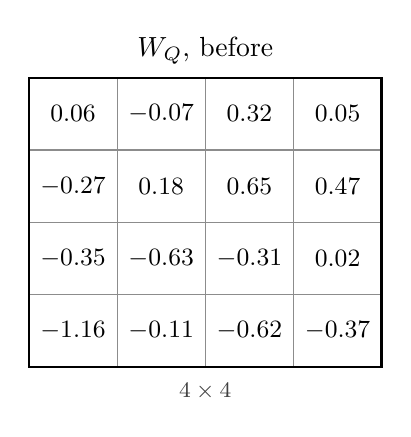
\begin{tikzpicture}
\draw[black!45, fill=white] (0.000,0.000) rectangle (1.120,-0.918);
\node[font=\small, text=black] at (0.560,-0.459) {$0.06$};
\draw[black!45, fill=white] (1.120,0.000) rectangle (2.240,-0.918);
\node[font=\small, text=black] at (1.680,-0.459) {$-0.07$};
\draw[black!45, fill=white] (2.240,0.000) rectangle (3.360,-0.918);
\node[font=\small, text=black] at (2.800,-0.459) {$0.32$};
\draw[black!45, fill=white] (3.360,0.000) rectangle (4.480,-0.918);
\node[font=\small, text=black] at (3.920,-0.459) {$0.05$};
\draw[black!45, fill=white] (0.000,-0.918) rectangle (1.120,-1.837);
\node[font=\small, text=black] at (0.560,-1.378) {$-0.27$};
\draw[black!45, fill=white] (1.120,-0.918) rectangle (2.240,-1.837);
\node[font=\small, text=black] at (1.680,-1.378) {$0.18$};
\draw[black!45, fill=white] (2.240,-0.918) rectangle (3.360,-1.837);
\node[font=\small, text=black] at (2.800,-1.378) {$0.65$};
\draw[black!45, fill=white] (3.360,-0.918) rectangle (4.480,-1.837);
\node[font=\small, text=black] at (3.920,-1.378) {$0.47$};
\draw[black!45, fill=white] (0.000,-1.837) rectangle (1.120,-2.755);
\node[font=\small, text=black] at (0.560,-2.296) {$-0.35$};
\draw[black!45, fill=white] (1.120,-1.837) rectangle (2.240,-2.755);
\node[font=\small, text=black] at (1.680,-2.296) {$-0.63$};
\draw[black!45, fill=white] (2.240,-1.837) rectangle (3.360,-2.755);
\node[font=\small, text=black] at (2.800,-2.296) {$-0.31$};
\draw[black!45, fill=white] (3.360,-1.837) rectangle (4.480,-2.755);
\node[font=\small, text=black] at (3.920,-2.296) {$0.02$};
\draw[black!45, fill=white] (0.000,-2.755) rectangle (1.120,-3.674);
\node[font=\small, text=black] at (0.560,-3.214) {$-1.16$};
\draw[black!45, fill=white] (1.120,-2.755) rectangle (2.240,-3.674);
\node[font=\small, text=black] at (1.680,-3.214) {$-0.11$};
\draw[black!45, fill=white] (2.240,-2.755) rectangle (3.360,-3.674);
\node[font=\small, text=black] at (2.800,-3.214) {$-0.62$};
\draw[black!45, fill=white] (3.360,-2.755) rectangle (4.480,-3.674);
\node[font=\small, text=black] at (3.920,-3.214) {$-0.37$};
\draw[line width=0.9pt] (0.000,0.000) rectangle (4.480,-3.674);
\node[anchor=south, font=\normalsize] at (2.240,0.050) {$W_Q$, before};
\node[anchor=north, font=\footnotesize, text=black!75] at (2.240,-3.754) {$4\times4$};
\end{tikzpicture}
\qquad
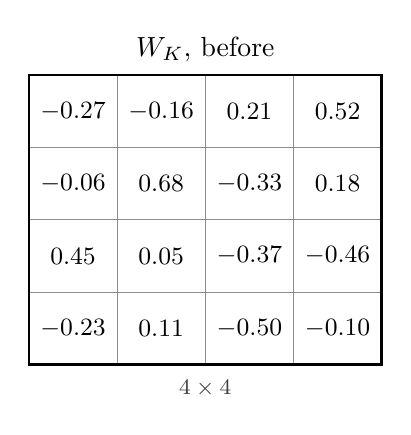
\begin{tikzpicture}
\draw[black!45, fill=white] (0.000,0.000) rectangle (1.120,-0.918);
\node[font=\small, text=black] at (0.560,-0.459) {$-0.27$};
\draw[black!45, fill=white] (1.120,0.000) rectangle (2.240,-0.918);
\node[font=\small, text=black] at (1.680,-0.459) {$-0.16$};
\draw[black!45, fill=white] (2.240,0.000) rectangle (3.360,-0.918);
\node[font=\small, text=black] at (2.800,-0.459) {$0.21$};
\draw[black!45, fill=white] (3.360,0.000) rectangle (4.480,-0.918);
\node[font=\small, text=black] at (3.920,-0.459) {$0.52$};
\draw[black!45, fill=white] (0.000,-0.918) rectangle (1.120,-1.837);
\node[font=\small, text=black] at (0.560,-1.378) {$-0.06$};
\draw[black!45, fill=white] (1.120,-0.918) rectangle (2.240,-1.837);
\node[font=\small, text=black] at (1.680,-1.378) {$0.68$};
\draw[black!45, fill=white] (2.240,-0.918) rectangle (3.360,-1.837);
\node[font=\small, text=black] at (2.800,-1.378) {$-0.33$};
\draw[black!45, fill=white] (3.360,-0.918) rectangle (4.480,-1.837);
\node[font=\small, text=black] at (3.920,-1.378) {$0.18$};
\draw[black!45, fill=white] (0.000,-1.837) rectangle (1.120,-2.755);
\node[font=\small, text=black] at (0.560,-2.296) {$0.45$};
\draw[black!45, fill=white] (1.120,-1.837) rectangle (2.240,-2.755);
\node[font=\small, text=black] at (1.680,-2.296) {$0.05$};
\draw[black!45, fill=white] (2.240,-1.837) rectangle (3.360,-2.755);
\node[font=\small, text=black] at (2.800,-2.296) {$-0.37$};
\draw[black!45, fill=white] (3.360,-1.837) rectangle (4.480,-2.755);
\node[font=\small, text=black] at (3.920,-2.296) {$-0.46$};
\draw[black!45, fill=white] (0.000,-2.755) rectangle (1.120,-3.674);
\node[font=\small, text=black] at (0.560,-3.214) {$-0.23$};
\draw[black!45, fill=white] (1.120,-2.755) rectangle (2.240,-3.674);
\node[font=\small, text=black] at (1.680,-3.214) {$0.11$};
\draw[black!45, fill=white] (2.240,-2.755) rectangle (3.360,-3.674);
\node[font=\small, text=black] at (2.800,-3.214) {$-0.50$};
\draw[black!45, fill=white] (3.360,-2.755) rectangle (4.480,-3.674);
\node[font=\small, text=black] at (3.920,-3.214) {$-0.10$};
\draw[line width=0.9pt] (0.000,0.000) rectangle (4.480,-3.674);
\node[anchor=south, font=\normalsize] at (2.240,0.050) {$W_K$, before};
\node[anchor=north, font=\footnotesize, text=black!75] at (2.240,-3.754) {$4\times4$};
\end{tikzpicture}
}\\[10pt]
\fitR{% AUTO-GENERATED by code/figlib.py helpers -- do not edit
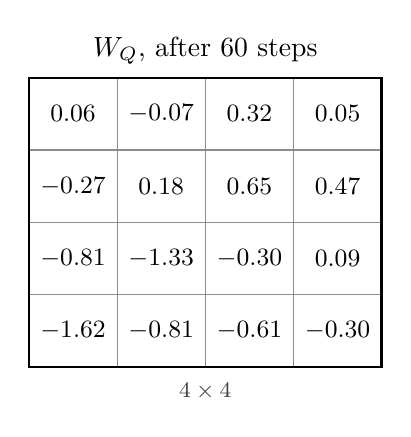
\begin{tikzpicture}
\draw[black!45, fill=white] (0.000,0.000) rectangle (1.120,-0.918);
\node[font=\small, text=black] at (0.560,-0.459) {$0.06$};
\draw[black!45, fill=white] (1.120,0.000) rectangle (2.240,-0.918);
\node[font=\small, text=black] at (1.680,-0.459) {$-0.07$};
\draw[black!45, fill=white] (2.240,0.000) rectangle (3.360,-0.918);
\node[font=\small, text=black] at (2.800,-0.459) {$0.32$};
\draw[black!45, fill=white] (3.360,0.000) rectangle (4.480,-0.918);
\node[font=\small, text=black] at (3.920,-0.459) {$0.05$};
\draw[black!45, fill=white] (0.000,-0.918) rectangle (1.120,-1.837);
\node[font=\small, text=black] at (0.560,-1.378) {$-0.27$};
\draw[black!45, fill=white] (1.120,-0.918) rectangle (2.240,-1.837);
\node[font=\small, text=black] at (1.680,-1.378) {$0.18$};
\draw[black!45, fill=white] (2.240,-0.918) rectangle (3.360,-1.837);
\node[font=\small, text=black] at (2.800,-1.378) {$0.65$};
\draw[black!45, fill=white] (3.360,-0.918) rectangle (4.480,-1.837);
\node[font=\small, text=black] at (3.920,-1.378) {$0.47$};
\draw[black!45, fill=white] (0.000,-1.837) rectangle (1.120,-2.755);
\node[font=\small, text=black] at (0.560,-2.296) {$-0.81$};
\draw[black!45, fill=white] (1.120,-1.837) rectangle (2.240,-2.755);
\node[font=\small, text=black] at (1.680,-2.296) {$-1.33$};
\draw[black!45, fill=white] (2.240,-1.837) rectangle (3.360,-2.755);
\node[font=\small, text=black] at (2.800,-2.296) {$-0.30$};
\draw[black!45, fill=white] (3.360,-1.837) rectangle (4.480,-2.755);
\node[font=\small, text=black] at (3.920,-2.296) {$0.09$};
\draw[black!45, fill=white] (0.000,-2.755) rectangle (1.120,-3.674);
\node[font=\small, text=black] at (0.560,-3.214) {$-1.62$};
\draw[black!45, fill=white] (1.120,-2.755) rectangle (2.240,-3.674);
\node[font=\small, text=black] at (1.680,-3.214) {$-0.81$};
\draw[black!45, fill=white] (2.240,-2.755) rectangle (3.360,-3.674);
\node[font=\small, text=black] at (2.800,-3.214) {$-0.61$};
\draw[black!45, fill=white] (3.360,-2.755) rectangle (4.480,-3.674);
\node[font=\small, text=black] at (3.920,-3.214) {$-0.30$};
\draw[line width=0.9pt] (0.000,0.000) rectangle (4.480,-3.674);
\node[anchor=south, font=\normalsize] at (2.240,0.050) {$W_Q$, after 60 steps};
\node[anchor=north, font=\footnotesize, text=black!75] at (2.240,-3.754) {$4\times4$};
\end{tikzpicture}
\qquad
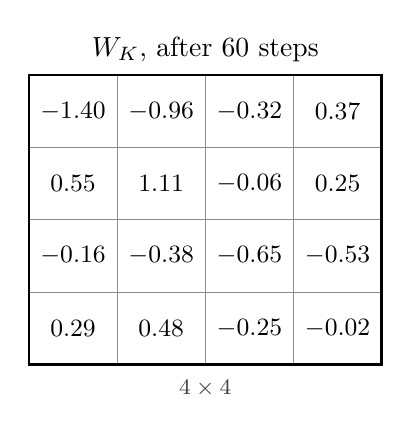
\begin{tikzpicture}
\draw[black!45, fill=white] (0.000,0.000) rectangle (1.120,-0.918);
\node[font=\small, text=black] at (0.560,-0.459) {$-1.40$};
\draw[black!45, fill=white] (1.120,0.000) rectangle (2.240,-0.918);
\node[font=\small, text=black] at (1.680,-0.459) {$-0.96$};
\draw[black!45, fill=white] (2.240,0.000) rectangle (3.360,-0.918);
\node[font=\small, text=black] at (2.800,-0.459) {$-0.32$};
\draw[black!45, fill=white] (3.360,0.000) rectangle (4.480,-0.918);
\node[font=\small, text=black] at (3.920,-0.459) {$0.37$};
\draw[black!45, fill=white] (0.000,-0.918) rectangle (1.120,-1.837);
\node[font=\small, text=black] at (0.560,-1.378) {$0.55$};
\draw[black!45, fill=white] (1.120,-0.918) rectangle (2.240,-1.837);
\node[font=\small, text=black] at (1.680,-1.378) {$1.11$};
\draw[black!45, fill=white] (2.240,-0.918) rectangle (3.360,-1.837);
\node[font=\small, text=black] at (2.800,-1.378) {$-0.06$};
\draw[black!45, fill=white] (3.360,-0.918) rectangle (4.480,-1.837);
\node[font=\small, text=black] at (3.920,-1.378) {$0.25$};
\draw[black!45, fill=white] (0.000,-1.837) rectangle (1.120,-2.755);
\node[font=\small, text=black] at (0.560,-2.296) {$-0.16$};
\draw[black!45, fill=white] (1.120,-1.837) rectangle (2.240,-2.755);
\node[font=\small, text=black] at (1.680,-2.296) {$-0.38$};
\draw[black!45, fill=white] (2.240,-1.837) rectangle (3.360,-2.755);
\node[font=\small, text=black] at (2.800,-2.296) {$-0.65$};
\draw[black!45, fill=white] (3.360,-1.837) rectangle (4.480,-2.755);
\node[font=\small, text=black] at (3.920,-2.296) {$-0.53$};
\draw[black!45, fill=white] (0.000,-2.755) rectangle (1.120,-3.674);
\node[font=\small, text=black] at (0.560,-3.214) {$0.29$};
\draw[black!45, fill=white] (1.120,-2.755) rectangle (2.240,-3.674);
\node[font=\small, text=black] at (1.680,-3.214) {$0.48$};
\draw[black!45, fill=white] (2.240,-2.755) rectangle (3.360,-3.674);
\node[font=\small, text=black] at (2.800,-3.214) {$-0.25$};
\draw[black!45, fill=white] (3.360,-2.755) rectangle (4.480,-3.674);
\node[font=\small, text=black] at (3.920,-3.214) {$-0.02$};
\draw[line width=0.9pt] (0.000,0.000) rectangle (4.480,-3.674);
\node[anchor=south, font=\normalsize] at (2.240,0.050) {$W_K$, after 60 steps};
\node[anchor=north, font=\footnotesize, text=black!75] at (2.240,-3.754) {$4\times4$};
\end{tikzpicture}
}
\captionof{figure}{The query machine $W_Q$ and the key machine $W_K$ before and after 60 good steps. Look at which numbers moved.
In $W_Q$ only rows 3 and 4 changed: the only query that matters here is \tok{time}'s, and its arrow
$(0,0,1,1)$ uses only those two rows (\S3.3), so rows 1 and 2 got no nudge at all. In $W_K$ every row moved,
because the three keys together use all four rows. None of the numbers was told about \tok{waste}.}
\end{minipage}\par\medskip

\par\medskip\noindent\begin{minipage}{\linewidth}\centering
\fitR{% AUTO-GENERATED by code/figlib.py helpers -- do not edit
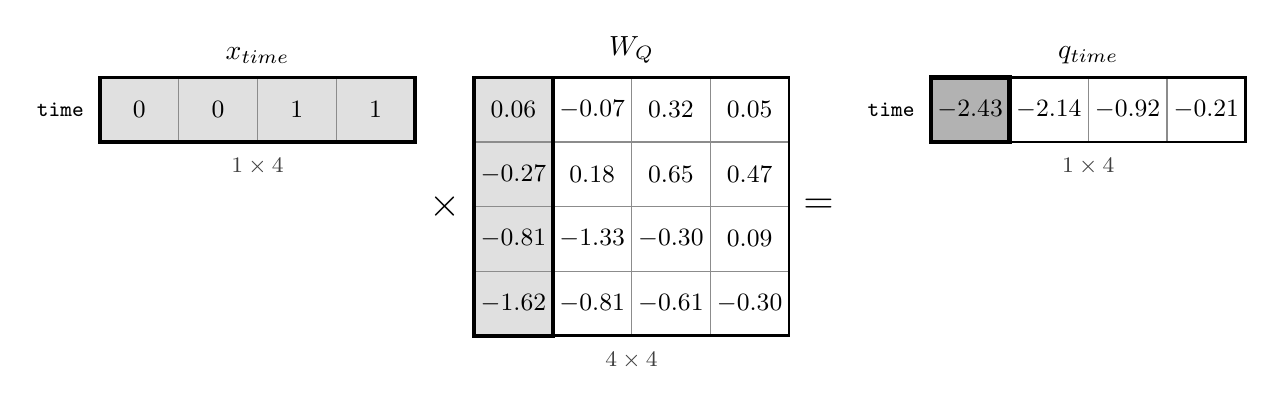
\begin{tikzpicture}
\draw[black!45, fill=black!12] (0.000,0.000) rectangle (1.000,-0.820);
\node[font=\small, text=black] at (0.500,-0.410) {$0$};
\draw[black!45, fill=black!12] (1.000,0.000) rectangle (2.000,-0.820);
\node[font=\small, text=black] at (1.500,-0.410) {$0$};
\draw[black!45, fill=black!12] (2.000,0.000) rectangle (3.000,-0.820);
\node[font=\small, text=black] at (2.500,-0.410) {$1$};
\draw[black!45, fill=black!12] (3.000,0.000) rectangle (4.000,-0.820);
\node[font=\small, text=black] at (3.500,-0.410) {$1$};
\draw[line width=1.4pt] (0.000,0.000) rectangle (4.000,-0.820);
\draw[line width=0.9pt] (0.000,0.000) rectangle (4.000,-0.820);
\node[anchor=east, font=\footnotesize\ttfamily] at (-0.080,-0.410) {time};
\node[anchor=south, font=\normalsize] at (2.000,0.050) {$\bm{x}_{\text{time}}$};
\node[anchor=north, font=\footnotesize, text=black!75] at (2.000,-0.900) {$1\times4$};
\draw[black!45, fill=black!12] (4.750,0.000) rectangle (5.750,-0.820);
\node[font=\small, text=black] at (5.250,-0.410) {$0.06$};
\draw[black!45, fill=white] (5.750,0.000) rectangle (6.750,-0.820);
\node[font=\small, text=black] at (6.250,-0.410) {$-0.07$};
\draw[black!45, fill=white] (6.750,0.000) rectangle (7.750,-0.820);
\node[font=\small, text=black] at (7.250,-0.410) {$0.32$};
\draw[black!45, fill=white] (7.750,0.000) rectangle (8.750,-0.820);
\node[font=\small, text=black] at (8.250,-0.410) {$0.05$};
\draw[black!45, fill=black!12] (4.750,-0.820) rectangle (5.750,-1.640);
\node[font=\small, text=black] at (5.250,-1.230) {$-0.27$};
\draw[black!45, fill=white] (5.750,-0.820) rectangle (6.750,-1.640);
\node[font=\small, text=black] at (6.250,-1.230) {$0.18$};
\draw[black!45, fill=white] (6.750,-0.820) rectangle (7.750,-1.640);
\node[font=\small, text=black] at (7.250,-1.230) {$0.65$};
\draw[black!45, fill=white] (7.750,-0.820) rectangle (8.750,-1.640);
\node[font=\small, text=black] at (8.250,-1.230) {$0.47$};
\draw[black!45, fill=black!12] (4.750,-1.640) rectangle (5.750,-2.460);
\node[font=\small, text=black] at (5.250,-2.050) {$-0.81$};
\draw[black!45, fill=white] (5.750,-1.640) rectangle (6.750,-2.460);
\node[font=\small, text=black] at (6.250,-2.050) {$-1.33$};
\draw[black!45, fill=white] (6.750,-1.640) rectangle (7.750,-2.460);
\node[font=\small, text=black] at (7.250,-2.050) {$-0.30$};
\draw[black!45, fill=white] (7.750,-1.640) rectangle (8.750,-2.460);
\node[font=\small, text=black] at (8.250,-2.050) {$0.09$};
\draw[black!45, fill=black!12] (4.750,-2.460) rectangle (5.750,-3.280);
\node[font=\small, text=black] at (5.250,-2.870) {$-1.62$};
\draw[black!45, fill=white] (5.750,-2.460) rectangle (6.750,-3.280);
\node[font=\small, text=black] at (6.250,-2.870) {$-0.81$};
\draw[black!45, fill=white] (6.750,-2.460) rectangle (7.750,-3.280);
\node[font=\small, text=black] at (7.250,-2.870) {$-0.61$};
\draw[black!45, fill=white] (7.750,-2.460) rectangle (8.750,-3.280);
\node[font=\small, text=black] at (8.250,-2.870) {$-0.30$};
\draw[line width=1.4pt] (4.750,0.000) rectangle (5.750,-3.280);
\draw[line width=0.9pt] (4.750,0.000) rectangle (8.750,-3.280);
\node[anchor=south, font=\normalsize] at (6.750,0.050) {$W_Q$};
\node[anchor=north, font=\footnotesize, text=black!75] at (6.750,-3.360) {$4\times4$};
\draw[black!45, fill=black!30] (10.550,0.000) rectangle (11.550,-0.820);
\node[font=\small, text=black] at (11.050,-0.410) {$-2.43$};
\draw[black!45, fill=white] (11.550,0.000) rectangle (12.550,-0.820);
\node[font=\small, text=black] at (12.050,-0.410) {$-2.14$};
\draw[black!45, fill=white] (12.550,0.000) rectangle (13.550,-0.820);
\node[font=\small, text=black] at (13.050,-0.410) {$-0.92$};
\draw[black!45, fill=white] (13.550,0.000) rectangle (14.550,-0.820);
\node[font=\small, text=black] at (14.050,-0.410) {$-0.21$};
\draw[line width=1.6pt] (10.550,0.000) rectangle (11.550,-0.820);
\draw[line width=0.9pt] (10.550,0.000) rectangle (14.550,-0.820);
\node[anchor=east, font=\footnotesize\ttfamily] at (10.470,-0.410) {time};
\node[anchor=south, font=\normalsize] at (12.550,0.050) {$\bm{q}_{\text{time}}$};
\node[anchor=north, font=\footnotesize, text=black!75] at (12.550,-0.900) {$1\times4$};
\node[font=\Large] at (4.375,-1.640) {$\times$};
\node[font=\Large] at (9.125,-1.640) {$=$};
\end{tikzpicture}
}\\[3pt]
% AUTO-GENERATED by code/ch*_figs.py -- do not edit
{\small highlighted row (\texttt{time}) $\cdot$ highlighted column (column 1): $(0)(0.06) + (0)(-0.27) + (1)(-0.81) + (1)(-1.62) = \mathbf{-2.43}$}
\\[10pt]
\fitR{% AUTO-GENERATED by code/figlib.py helpers -- do not edit
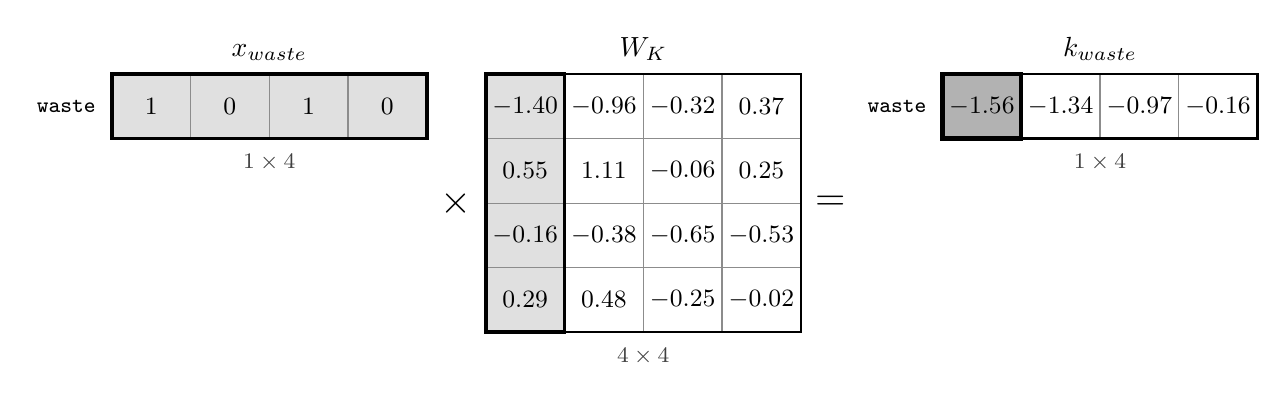
\begin{tikzpicture}
\draw[black!45, fill=black!12] (0.000,0.000) rectangle (1.000,-0.820);
\node[font=\small, text=black] at (0.500,-0.410) {$1$};
\draw[black!45, fill=black!12] (1.000,0.000) rectangle (2.000,-0.820);
\node[font=\small, text=black] at (1.500,-0.410) {$0$};
\draw[black!45, fill=black!12] (2.000,0.000) rectangle (3.000,-0.820);
\node[font=\small, text=black] at (2.500,-0.410) {$1$};
\draw[black!45, fill=black!12] (3.000,0.000) rectangle (4.000,-0.820);
\node[font=\small, text=black] at (3.500,-0.410) {$0$};
\draw[line width=1.4pt] (0.000,0.000) rectangle (4.000,-0.820);
\draw[line width=0.9pt] (0.000,0.000) rectangle (4.000,-0.820);
\node[anchor=east, font=\footnotesize\ttfamily] at (-0.080,-0.410) {waste};
\node[anchor=south, font=\normalsize] at (2.000,0.050) {$\bm{x}_{\text{waste}}$};
\node[anchor=north, font=\footnotesize, text=black!75] at (2.000,-0.900) {$1\times4$};
\draw[black!45, fill=black!12] (4.750,0.000) rectangle (5.750,-0.820);
\node[font=\small, text=black] at (5.250,-0.410) {$-1.40$};
\draw[black!45, fill=white] (5.750,0.000) rectangle (6.750,-0.820);
\node[font=\small, text=black] at (6.250,-0.410) {$-0.96$};
\draw[black!45, fill=white] (6.750,0.000) rectangle (7.750,-0.820);
\node[font=\small, text=black] at (7.250,-0.410) {$-0.32$};
\draw[black!45, fill=white] (7.750,0.000) rectangle (8.750,-0.820);
\node[font=\small, text=black] at (8.250,-0.410) {$0.37$};
\draw[black!45, fill=black!12] (4.750,-0.820) rectangle (5.750,-1.640);
\node[font=\small, text=black] at (5.250,-1.230) {$0.55$};
\draw[black!45, fill=white] (5.750,-0.820) rectangle (6.750,-1.640);
\node[font=\small, text=black] at (6.250,-1.230) {$1.11$};
\draw[black!45, fill=white] (6.750,-0.820) rectangle (7.750,-1.640);
\node[font=\small, text=black] at (7.250,-1.230) {$-0.06$};
\draw[black!45, fill=white] (7.750,-0.820) rectangle (8.750,-1.640);
\node[font=\small, text=black] at (8.250,-1.230) {$0.25$};
\draw[black!45, fill=black!12] (4.750,-1.640) rectangle (5.750,-2.460);
\node[font=\small, text=black] at (5.250,-2.050) {$-0.16$};
\draw[black!45, fill=white] (5.750,-1.640) rectangle (6.750,-2.460);
\node[font=\small, text=black] at (6.250,-2.050) {$-0.38$};
\draw[black!45, fill=white] (6.750,-1.640) rectangle (7.750,-2.460);
\node[font=\small, text=black] at (7.250,-2.050) {$-0.65$};
\draw[black!45, fill=white] (7.750,-1.640) rectangle (8.750,-2.460);
\node[font=\small, text=black] at (8.250,-2.050) {$-0.53$};
\draw[black!45, fill=black!12] (4.750,-2.460) rectangle (5.750,-3.280);
\node[font=\small, text=black] at (5.250,-2.870) {$0.29$};
\draw[black!45, fill=white] (5.750,-2.460) rectangle (6.750,-3.280);
\node[font=\small, text=black] at (6.250,-2.870) {$0.48$};
\draw[black!45, fill=white] (6.750,-2.460) rectangle (7.750,-3.280);
\node[font=\small, text=black] at (7.250,-2.870) {$-0.25$};
\draw[black!45, fill=white] (7.750,-2.460) rectangle (8.750,-3.280);
\node[font=\small, text=black] at (8.250,-2.870) {$-0.02$};
\draw[line width=1.4pt] (4.750,0.000) rectangle (5.750,-3.280);
\draw[line width=0.9pt] (4.750,0.000) rectangle (8.750,-3.280);
\node[anchor=south, font=\normalsize] at (6.750,0.050) {$W_K$};
\node[anchor=north, font=\footnotesize, text=black!75] at (6.750,-3.360) {$4\times4$};
\draw[black!45, fill=black!30] (10.550,0.000) rectangle (11.550,-0.820);
\node[font=\small, text=black] at (11.050,-0.410) {$-1.56$};
\draw[black!45, fill=white] (11.550,0.000) rectangle (12.550,-0.820);
\node[font=\small, text=black] at (12.050,-0.410) {$-1.34$};
\draw[black!45, fill=white] (12.550,0.000) rectangle (13.550,-0.820);
\node[font=\small, text=black] at (13.050,-0.410) {$-0.97$};
\draw[black!45, fill=white] (13.550,0.000) rectangle (14.550,-0.820);
\node[font=\small, text=black] at (14.050,-0.410) {$-0.16$};
\draw[line width=1.6pt] (10.550,0.000) rectangle (11.550,-0.820);
\draw[line width=0.9pt] (10.550,0.000) rectangle (14.550,-0.820);
\node[anchor=east, font=\footnotesize\ttfamily] at (10.470,-0.410) {waste};
\node[anchor=south, font=\normalsize] at (12.550,0.050) {$\bm{k}_{\text{waste}}$};
\node[anchor=north, font=\footnotesize, text=black!75] at (12.550,-0.900) {$1\times4$};
\node[font=\Large] at (4.375,-1.640) {$\times$};
\node[font=\Large] at (9.125,-1.640) {$=$};
\end{tikzpicture}
}\\[3pt]
% AUTO-GENERATED by code/ch*_figs.py -- do not edit
{\small highlighted row (\texttt{waste}) $\cdot$ highlighted column (column 1): $(1)(-1.40) + (0)(0.55) + (1)(-0.16) + (0)(0.29) = \mathbf{-1.56}$}

\captionof{figure}{After training: \tok{time}'s arrow times the trained $W_Q$ gives its query, and \tok{waste}'s arrow
times the trained $W_K$ gives its key. One row times one column per number, as always; the highlighted cell is
worked out underneath each product.}
\end{minipage}\par\medskip

The query turned by about \nEightTurned\ degrees towards \tok{waste}'s key and grew longer. That is \S3.10 exactly:
turned towards the key that helps, and stretched to be more decisive. Nobody told the model to look at
\tok{waste}. The only instruction was ``make the surprise at \tok{Sorry} smaller'', and attending to
\tok{waste} turned out to be the way downhill. Why that way? Look at \tok{waste}'s value arrow in our
original toy: $(1,1,0,0)$, the very same arrow as \tok{Sorry}'s embedding. Handing it over pushes the
output towards \tok{Sorry}.

The slow run (learning rate \nEightTrainSlowLr) is going the same way but has only reached a share of
\nEightTrainSlowShareEnd\ and a loss of \nEightTrainSlowLossEnd.

Now look at the wild run (learning rate \nEightTrainWildLr). Its loss is \nEightTrainWildLossEnd: perfect!
Yet \tok{time} gives \tok{waste} a share of only \nEightTrainWildShareEnd, and the query points
\nEightTrainWildAngEnd$^\circ$ away from \tok{waste}'s key. Giant steps found a different valley: they changed
what the other tokens hand over until \tok{Sorry} came out anyway. On this one exercise that works. On any new
sentence, a model that ignores \tok{waste} is useless. This is our first look at a problem \S8.6 measures
properly: a low loss on the exercises you trained on does not mean the model learned what you hoped.

\begin{wrongidea}{8.4}
\emph{``Training adjusts each word's arrow inside the sentence.''} Nothing in the runs above touched an arrow
directly. Only the numbers in $W_Q$, $W_K$, $W_V$ changed; the arrows moved because the machines that make
them changed. That is why learning transfers: the same machine also makes the arrows for \tok{waste of
money}.
\end{wrongidea}

\begin{wrongidea}{8.8}
\emph{``A low training loss means the model learned what we wanted.''} The wild run has the lowest loss of
all three and the worst attention. Loss measures only the exercises it was given.
\end{wrongidea}

\begin{checkq}
In the good run, which change made the model attend to \tok{waste}?
\begin{options}
\item We instructed it to look at \tok{waste}.
\item Steps that lowered the surprise at \tok{Sorry} happened to turn the query towards \tok{waste}'s key.
\item The arrow of \tok{waste} was moved closer to the arrow of \tok{time}.
\item The loss reached zero, which forces attention onto the most useful word.
\end{options}
\end{checkq}

\Summary{trained only to reduce surprise, the toy's query for \tok{time} turned from
\nEightTrainAngStart$^\circ$ to \nEightTrainGoodAngEnd$^\circ$ off \tok{waste}'s key and grew longer, while
a run with steps that were too big found a zero loss that ignores \tok{waste}.}

%---------------------------------------------------------------------
\subsection*{8.5\quad Batches, noise, and a smarter walker}

\Predict A real dataset has billions of exercises. Computing the exact downhill direction would mean running
all of them before every single step. What if you used only a handful of exercises per step instead? Would
the direction still be any good?

\Picture You are lost in a town and ask for directions. One passer-by points roughly the right way, but might
be off. Ask eight people and average their arrows, and the average points much more reliably. Each person is
one exercise; their arrow is the downhill direction for that exercise alone.

Let us measure it on our nine exercises (\S8.2), from the random start of \S8.4. For each batch size we draw
300 random batches, compute their downhill direction, and compare it with the direction from all nine
exercises, using the agreement of two arrows from \S3.2 ($\cos$ of the angle between them; 1 means identical):

\begin{center}
\small
\begin{tabular}{@{}l c c c c@{}}
\toprule
exercises per batch & 1 & 2 & 4 & 8\\
average agreement with the full direction & \nEightBatchCosOne & \nEightBatchCosTwo & \nEightBatchCosFour & \nEightBatchCosEight\\
\bottomrule
\end{tabular}
\end{center}
One exercise points, on average, about \nEightBatchAngOne$^\circ$ away from the full direction; eight
point about \nEightBatchAngEight$^\circ$ away. Each step is noisy, but noisy steps that are right on average
still go downhill on average, and they are thousands of times cheaper. This is \emph{stochastic gradient
descent} (its roots are in Robbins and Monro, 1951). Do you see the coin tosses of \S3.8 again? Averaging
$n$ noisy arrows cuts the noise roughly like $1/\sqrt{n}$, the same square-root rule.

\Exactly Each step: pick a batch of exercises, compute the average gradient $\bm{g}_{\text{batch}}$ over that
batch only, and update $\bm{\theta}\leftarrow\bm{\theta}-\eta\,\bm{g}_{\text{batch}}$.

\paragraph{A smarter walker: Adam.} Plain steps have two weaknesses. On a long, gently sloping valley floor
they creep; and when some knobs are steep and others nearly flat, one learning rate is too big for the first
and too small for the second. Adam (Kingma and Ba, 2015) fixes both with two memories. It keeps a running
average of recent directions, so consistent directions build up speed and noisy ones cancel (like a heavy
ball rolling downhill). And it keeps a running average of how large each knob's slope has been, and divides
by it, so every knob takes steps of similar size, steep or flat. On our tiny toy it is not faster: plain steps
reach a loss below 0.1 after \nEightSgdSteps\ steps and Adam after \nEightAdamSteps. Its advantage shows on
large models, where knobs differ in steepness by many factors of ten. Nearly every model in Chapter 10 was
trained with Adam or its variant AdamW (Loshchilov and Hutter, 2019).

\begin{breaks}
The passers-by picture assumes every exercise is equally trustworthy and independent. Real batches are not:
nearby text is similar, and some exercises are far more frequent than others. Also, the noise is not only a
cost. Keskar and colleagues (2017) found that small, noisy batches tend to end in wider valleys, which carry over
better to new text; how much this matters for large models is still debated.
\end{breaks}

\Why Why accept noisy steps at all? Because the exact direction costs a pass over the entire dataset, and
by the time you had it, a noisy walker would have taken thousands of steps. Cheap, roughly right, and often
beats expensive and exact.

\begin{wrongidea}{8.6}
\emph{``Each step on a batch moves exactly downhill on the whole dataset.''} With one exercise per batch,
the direction is off by about \nEightBatchAngOne$^\circ$ on average. A training step is a vote by a few
exercises, not the verdict of all of them.
\end{wrongidea}

\begin{checkq}
Doubling the batch size from 4 to 8 exercises changes the average agreement from \nEightBatchCosFour\ to
\nEightBatchCosEight. What does that mean?
\begin{options}
\item Each step is now exactly downhill.
\item Each step's direction is closer to the full-data direction, at twice the cost per step.
\item The learning rate has doubled.
\item The loss is now twice as small.
\end{options}
\end{checkq}

\Summary{real training steps use small random batches, whose directions are noisy but right on average, and
Adam smooths the direction and evens out the step size across knobs.}

%---------------------------------------------------------------------
\subsection*{8.6\quad A real run: a tiny transformer learns from real text}

\Predict Our real model reads text one character at a time. The text is a corpus of transcribed technical
talks on AI engineering, split into nine parts. It uses \nEightRunV\ different
characters (letters, digits, space and a little punctuation). Before any training, the model knows nothing.
What loss should it start with? (Hint: the know-nothing model of \S8.1.)

Everything from Chapters 3 to 8 now runs together, at a size a laptop can handle:
\begin{itemize}
\item characters as tokens (\nEightRunV\ of them), each with an arrow of $d=64$ numbers, plus a learned
position arrow (Chapter 4);
\item two blocks, each with 2 attention heads and an MLP (Chapters 5 and 6), \nEightRunParams\ knobs in all,
with the output scores tied to the embedding table as in our toy;
\item training text: parts 1--8 (\nEightRunTrainChars\ characters); held-out text, never trained on:
part 9 (\nEightRunValChars\ characters);
\item \nEightRunSteps\ steps of AdamW, each on a batch of 32 pieces of 64 characters: \nEightRunTokensSeen\
next-character exercises in total;
\item one CPU thread and fixed random seeds, so running \texttt{code/ch8\_train.py} again gives identical
numbers.
\end{itemize}

\Sanity A know-nothing guess over \nEightRunV\ characters has loss $\ln \nEightRunV = \nEightRunUniform$. Our
model starts at \nEightRunLossStart, close to that, as it should. My first attempt did not: with the default
starting weights of the software library, the starting loss was \nEightRunBadInit, ten times worse than
guessing. That one number said something was broken before a single step was taken. (The cause: with the
output tied to large starting embeddings, every character's arrow agreed strongly with itself, so the model
began confidently repeating whatever it had last seen. Starting the embeddings small, with spread 0.02 as in
Radford and colleagues' first GPT, 2018, fixed it.) \emph{Always check the starting loss against the
know-nothing value.}

\par\medskip\noindent\begin{minipage}{\linewidth}\centering
\begin{tikzpicture}
\begin{axis}[width=12cm, height=5.2cm, xmin=0, xmax=2500, ymin=1, ymax=4, xlabel={training step},
  ylabel={loss (per character)}, label style={font=\small}, tick label style={font=\footnotesize},
  axis lines*=left, scaled x ticks=false, xtick={0,500,1000,1500,2000,2500}]
\addplot[black, thick, no marks] table[x=step, y=train] {data_ch8/curve.dat};
\addplot[black!50, thick, dashed, no marks] table[x=step, y=val] {data_ch8/curve.dat};
\addplot[black!60, densely dotted, thick, no marks, domain=0:2500] {\nEightRunUniform};
\node[font=\footnotesize, anchor=south west] at (axis cs:1500,\nEightRunUniform) {know-nothing guess, $\ln \nEightRunV$};
\node[font=\footnotesize, anchor=west] at (axis cs:1300,3.05) {solid: parts 1--8 (trained on)};
\node[font=\footnotesize, anchor=west] at (axis cs:1300,2.75) {dashed: part 9 (held out)};
\end{axis}
\end{tikzpicture}
\captionof{figure}{The real loss curve of our tiny transformer, measured every 100 steps.}
\end{minipage}\par\medskip

After \nEightRunSteps\ steps the loss is \nEightRunLossEnd\ on the training text and \nEightRunValEnd\ on
part 9, which it never saw. A loss is easier to feel as a \emph{perplexity}, $e^{\text{loss}}$: the model
is as unsure as if it were choosing evenly among that many characters. It started at
\nEightRunPplStart\ and ended at \nEightRunPplEnd. Here is what the model writes after the prompt
\tok{waste of time}, at three moments (same random seed for the sampling each time):

\begin{plainbox}
\small\raggedright
\noindent\textbf{step \nEightSampleZeroStep:}\ \texttt{\nEightSampleZero}\\[3pt]
\textbf{step \nEightSampleMidStep:}\ \texttt{\nEightSampleMid}\\[3pt]
\textbf{step \nEightSampleEndStep:}\ \texttt{\nEightSampleEnd}
\end{plainbox}
At step 0 it is noise. By the end it writes words, spaces, full stops, and a phrase that the talks use often:
\emph{for example, if you}. It has never been told what a word is. Everything it knows came from
nudging \nEightRunParams\ knobs downhill on next-character surprise.

\paragraph{When the loss lies: overfitting.} Now train the same model on a tiny slice, the first
\nEightOverSmall\ characters of the corpus, for \nEightOverSteps\ steps.

\par\medskip\noindent\begin{minipage}{\linewidth}\centering
\begin{tikzpicture}
\begin{axis}[width=12cm, height=4.8cm, xmin=0, xmax=1200, ymin=0, ymax=6.5, xlabel={training step},
  ylabel={loss}, label style={font=\small}, tick label style={font=\footnotesize}, axis lines*=left, scaled x ticks=false]
\addplot[black, thick, no marks] table[x=step, y=train] {data_ch8/overfit.dat};
\addplot[black!50, thick, dashed, no marks] table[x=step, y=val] {data_ch8/overfit.dat};
\node[font=\footnotesize, anchor=west] at (axis cs:430,2.2) {dashed: held-out part 9, getting worse};
\node[font=\footnotesize, anchor=west] at (axis cs:430,1.5) {solid: the \nEightOverSmall\ characters it trains on};
\end{axis}
\end{tikzpicture}
\captionof{figure}{Overfitting, measured. Held-out loss is best at step \nEightOverBestStep\ (\nEightOverBestVal) and
then rises while training loss keeps falling.}
\end{minipage}\par\medskip

The training loss falls to \nEightOverTrainEnd: the model has nearly memorised those \nEightOverSmall\
characters. The loss on part 9 is best at step \nEightOverBestStep\ and then climbs to \nEightOverValEnd,
worse than guessing. It is the wild run of \S8.4 again, at full size.

\Picture A student who memorises last year's answer key scores full marks on last year's paper and fails
this year's. A student who learns the method does a little worse on last year's paper and well on this
year's. The held-out text is this year's paper. To learn the method instead of the answers, a model needs
enough training text with patterns that repeat.

\begin{breaks}
The exam picture suggests memorising is always bad. Large language models do memorise some text, and some
of that is useful (facts, names, code idioms). The problem is memorising \emph{instead of} learning patterns
that carry over, and the only way to tell the two apart is a held-out measurement.
\end{breaks}

\Why This is why every training run in this book reports two curves. The training curve tells you whether
the walker is going downhill. Only the held-out curve tells you whether downhill is where you wanted to go.
It is the same reason a fraud model is checked on transactions it was not trained on.

\begin{checkq}
Training loss is falling but held-out loss has started rising. Which reading is right?
\begin{options}
\item The model is improving; training loss is what counts.
\item The model is starting to memorise its training text; it is time to stop, add data, or shrink the model.
\item The learning rate is too small.
\item Held-out loss always rises at the end; ignore it.
\end{options}
\end{checkq}

\Summary{a real \nEightRunParams-knob transformer, trained on next-character surprise alone, went from noise
to word-like text with a held-out perplexity of \nEightRunPplEnd, and a run on too little text showed
training loss falling while held-out loss rose.}

%---------------------------------------------------------------------
\begin{principle}{learning is a loop of guess, surprise, small correction}
Strip away the transformer and this chapter describes a loop: make a prediction, measure how surprised you
should be by what actually happened, nudge your settings a little in the direction that would have reduced
the surprise, repeat on fresh cases, and keep some cases aside to check that the nudges carry over. The same
loop runs whenever you improve an agent's prompts against an evaluation set, tune a retriever on past
queries, or adjust a decision rule from outcomes. So does its failure: tune against the same evaluation
cases for long enough and you overfit to them, exactly like the \nEightOverSmall-character run. The defence
is the same too: a held-out set you do not tune against.
\end{principle}

\begin{lookingback}
\begin{enumerate}[label=(\arabic*),leftmargin=1.6em]
\item (Chapter 1) A sentence's probability is a product of next-word probabilities. What does the loss of
this chapter do to that product, and why does it matter for a computer?
\item (Chapter 3) Why did dividing scores by $\sqrt{d_k}$ matter for learning, not only for the starting
shares? (Appendix A, \S A.5, measures it.)
\item (Chapter 3) Which part of attention lets one pass over \nEightSeqLen\ tokens give \nEightNumEx\ honest
exercises?
\end{enumerate}
\end{lookingback}

\subsection*{Exercises}

\begin{exercise}
A model gives the right next word a probability of 0.25. What is the surprise? Compare it with the
know-nothing loss for a vocabulary of 12 words, and say which is better.
\end{exercise}

\begin{exercise}
A training step uses a batch of 32 sequences, each 64 tokens long. How many next-token exercises does one
step contain? Which idea from Chapter 3 makes that possible?
\end{exercise}

\begin{exercise}
In \S8.3, the slope at $90^\circ$ is \nEightSlopeNinety\ loss per degree. Using the update rule, how far does
the first step of the good walker (learning rate \nEightLrGood) move the angle? Check your answer against the
text.
\end{exercise}

\begin{exercise}
The wild run of \S8.4 reached a loss of \nEightTrainWildLossEnd\ while ignoring \tok{waste}. Describe one
measurement that would have caught this before you shipped the model.
\end{exercise}

\begin{exercise}
You train a model for a support team. Training loss keeps falling; held-out loss is lowest at step 200 and
rises after. Give three different things you could change, and say what each assumes about the cause.
\end{exercise}

\subsection*{Answers to Chapter 8}

\paragraph{Check yourself 8.1.} (b): $-\ln 0.5 = \nEightSurpHalf$. (a) reads the loss as the share of wrong
probability (M8.1). (c) scores only the top answer, like a test (M8.1); the loss would still be
\nEightSurpHalf\ because half the probability went elsewhere. (d) subtracts prediction from answer as for a
price (M8.2), which has no meaning for words, and a surprise can never be negative.

\paragraph{Check yourself 8.2.} (b). The mask hides every later token from row 3. (a) is false: \tok{Sorry}
is not the top word (\tok{\nEightTopWord} is). (c) is true but irrelevant: the equality holds for any weights.
(d) is M8.5: there are nine exercises in that one pass, not one.

\paragraph{Check yourself 8.3.} (b). Lower is to the right, so step right, by an amount proportional to how
steep it is. (a) climbs uphill. (c) is M8.3: too large a step overshoots. (d) confuses ``one side is lower''
with ``this is the bottom'' (M8.7); at the bottom, both sides are higher.

\paragraph{Check yourself 8.4.} (b). No one instructed the model (a). Arrows are never moved directly; the
machines change (c is M8.4). (d) is M8.8: the wild run reached zero loss while ignoring \tok{waste}.

\paragraph{Check yourself 8.5.} (b). More exercises per step give a direction that agrees better with the
full data, and each step costs more. (a) is M8.6: still not exact. (c) and (d) mix up batch size with the
learning rate and with the loss.

\paragraph{Check yourself 8.6.} (b). (a) is M8.8. (c) does not follow: a too-small learning rate shows up as
both curves falling slowly. (d) is false: on enough data, as in the main run, both curves fall together.

\paragraph{Exercise 8.1.} $-\ln 0.25 = \nEightExQuarter$. The know-nothing loss is $\ln 12 =
\nEightUniformLoss$, so $0.25$ on the right word is better: smaller surprise.

\paragraph{Exercise 8.2.} $32\times64=\nEightExBatchPreds$ exercises. The causal mask (\S3.6, Step 3) lets
every position be an honest exercise in the same pass.

\paragraph{Exercise 8.3.} Step $=$ learning rate $\times$ slope $= \nEightLrGood\times\nEightSlopeNinety
\approx \nEightExSlopeTimesLr$ degrees, from $90^\circ$ down to about $\nEightGoodFirst^\circ$, as in the text.

\paragraph{Exercise 8.4.} Measure the attention on a different sentence that also needs \tok{waste} (for
example \tok{waste of money}), or measure loss on held-out exercises. A model that solved one exercise by
memorising fails both checks.

\paragraph{Exercise 8.5.} Any three of: stop at the step with the best held-out loss (assumes later steps
only memorise); add more, varied training text (assumes too little data); use a smaller model (assumes too
many knobs for the data); lower the learning rate or add regularisation (assumes the walker is jumping into a
memorising valley). A good answer says which assumption it is testing.

\paragraph{What you now know.}
\begin{itemize}
\item The loss is the average surprise $-\ln p$ at the right next word; it rewards moving probability towards
the right word, and logs turn the chain of Chapter 1 into a sum.
\item Thanks to the mask, one pass gives an exercise at every position.
\item Training is walking downhill on the loss landscape, with a learning rate that must be neither too small
nor too large.
\item Trained only on surprise, the toy's query turned from \nEightTrainAngStart$^\circ$ to
\nEightTrainGoodAngEnd$^\circ$ off \tok{waste}'s key: the arrows of Chapter 3 really do turn and stretch.
\item Real steps use noisy batches; Adam smooths and evens out the steps.
\item A real tiny transformer learned word-like text from a corpus of talks, and a held-out curve is the only
way to see overfitting.
\end{itemize}
